% Options for packages loaded elsewhere
\PassOptionsToPackage{unicode}{hyperref}
\PassOptionsToPackage{hyphens}{url}
%
\documentclass[
  man]{apa6}
\usepackage{amsmath,amssymb}
\usepackage{iftex}
\ifPDFTeX
  \usepackage[T1]{fontenc}
  \usepackage[utf8]{inputenc}
  \usepackage{textcomp} % provide euro and other symbols
\else % if luatex or xetex
  \usepackage{unicode-math} % this also loads fontspec
  \defaultfontfeatures{Scale=MatchLowercase}
  \defaultfontfeatures[\rmfamily]{Ligatures=TeX,Scale=1}
\fi
\usepackage{lmodern}
\ifPDFTeX\else
  % xetex/luatex font selection
  \setmainfont[]{Arial}
\fi
% Use upquote if available, for straight quotes in verbatim environments
\IfFileExists{upquote.sty}{\usepackage{upquote}}{}
\IfFileExists{microtype.sty}{% use microtype if available
  \usepackage[]{microtype}
  \UseMicrotypeSet[protrusion]{basicmath} % disable protrusion for tt fonts
}{}
\makeatletter
\@ifundefined{KOMAClassName}{% if non-KOMA class
  \IfFileExists{parskip.sty}{%
    \usepackage{parskip}
  }{% else
    \setlength{\parindent}{0pt}
    \setlength{\parskip}{6pt plus 2pt minus 1pt}}
}{% if KOMA class
  \KOMAoptions{parskip=half}}
\makeatother
\usepackage{xcolor}
\usepackage{graphicx}
\makeatletter
\def\maxwidth{\ifdim\Gin@nat@width>\linewidth\linewidth\else\Gin@nat@width\fi}
\def\maxheight{\ifdim\Gin@nat@height>\textheight\textheight\else\Gin@nat@height\fi}
\makeatother
% Scale images if necessary, so that they will not overflow the page
% margins by default, and it is still possible to overwrite the defaults
% using explicit options in \includegraphics[width, height, ...]{}
\setkeys{Gin}{width=\maxwidth,height=\maxheight,keepaspectratio}
% Set default figure placement to htbp
\makeatletter
\def\fps@figure{htbp}
\makeatother
\setlength{\emergencystretch}{3em} % prevent overfull lines
\providecommand{\tightlist}{%
  \setlength{\itemsep}{0pt}\setlength{\parskip}{0pt}}
\setcounter{secnumdepth}{-\maxdimen} % remove section numbering
% Make \paragraph and \subparagraph free-standing
\ifx\paragraph\undefined\else
  \let\oldparagraph\paragraph
  \renewcommand{\paragraph}[1]{\oldparagraph{#1}\mbox{}}
\fi
\ifx\subparagraph\undefined\else
  \let\oldsubparagraph\subparagraph
  \renewcommand{\subparagraph}[1]{\oldsubparagraph{#1}\mbox{}}
\fi
\newlength{\cslhangindent}
\setlength{\cslhangindent}{1.5em}
\newlength{\csllabelwidth}
\setlength{\csllabelwidth}{3em}
\newlength{\cslentryspacingunit} % times entry-spacing
\setlength{\cslentryspacingunit}{\parskip}
\newenvironment{CSLReferences}[2] % #1 hanging-ident, #2 entry spacing
 {% don't indent paragraphs
  \setlength{\parindent}{0pt}
  % turn on hanging indent if param 1 is 1
  \ifodd #1
  \let\oldpar\par
  \def\par{\hangindent=\cslhangindent\oldpar}
  \fi
  % set entry spacing
  \setlength{\parskip}{#2\cslentryspacingunit}
 }%
 {}
\usepackage{calc}
\newcommand{\CSLBlock}[1]{#1\hfill\break}
\newcommand{\CSLLeftMargin}[1]{\parbox[t]{\csllabelwidth}{#1}}
\newcommand{\CSLRightInline}[1]{\parbox[t]{\linewidth - \csllabelwidth}{#1}\break}
\newcommand{\CSLIndent}[1]{\hspace{\cslhangindent}#1}
\ifLuaTeX
\usepackage[bidi=basic]{babel}
\else
\usepackage[bidi=default]{babel}
\fi
\babelprovide[main,import]{english}
\ifPDFTeX
\else
\babelfont[english]{rm}{Arial}
\fi
% get rid of language-specific shorthands (see #6817):
\let\LanguageShortHands\languageshorthands
\def\languageshorthands#1{}
\usepackage{pdflscape}
\DeclareDelayedFloatFlavor{landscape}{table}
\newcommand{\blandscape}{\begin{landscape}}
\newcommand{\elandscape}{\end{landscape}}
% Manuscript styling
\usepackage{upgreek}
\captionsetup{font=singlespacing,justification=justified}

% Table formatting
\usepackage{longtable}
\usepackage{lscape}
% \usepackage[counterclockwise]{rotating}   % Landscape page setup for large tables
\usepackage{multirow}		% Table styling
\usepackage{tabularx}		% Control Column width
\usepackage[flushleft]{threeparttable}	% Allows for three part tables with a specified notes section
\usepackage{threeparttablex}            % Lets threeparttable work with longtable

% Create new environments so endfloat can handle them
% \newenvironment{ltable}
%   {\begin{landscape}\centering\begin{threeparttable}}
%   {\end{threeparttable}\end{landscape}}
\newenvironment{lltable}{\begin{landscape}\centering\begin{ThreePartTable}}{\end{ThreePartTable}\end{landscape}}

% Enables adjusting longtable caption width to table width
% Solution found at http://golatex.de/longtable-mit-caption-so-breit-wie-die-tabelle-t15767.html
\makeatletter
\newcommand\LastLTentrywidth{1em}
\newlength\longtablewidth
\setlength{\longtablewidth}{1in}
\newcommand{\getlongtablewidth}{\begingroup \ifcsname LT@\roman{LT@tables}\endcsname \global\longtablewidth=0pt \renewcommand{\LT@entry}[2]{\global\advance\longtablewidth by ##2\relax\gdef\LastLTentrywidth{##2}}\@nameuse{LT@\roman{LT@tables}} \fi \endgroup}

% \setlength{\parindent}{0.5in}
% \setlength{\parskip}{0pt plus 0pt minus 0pt}

% Overwrite redefinition of paragraph and subparagraph by the default LaTeX template
% See https://github.com/crsh/papaja/issues/292
\makeatletter
\renewcommand{\paragraph}{\@startsection{paragraph}{4}{\parindent}%
  {0\baselineskip \@plus 0.2ex \@minus 0.2ex}%
  {-1em}%
  {\normalfont\normalsize\bfseries\itshape\typesectitle}}

\renewcommand{\subparagraph}[1]{\@startsection{subparagraph}{5}{1em}%
  {0\baselineskip \@plus 0.2ex \@minus 0.2ex}%
  {-\z@\relax}%
  {\normalfont\normalsize\itshape\hspace{\parindent}{#1}\textit{\addperi}}{\relax}}
\makeatother

\makeatletter
\usepackage{etoolbox}
\patchcmd{\maketitle}
  {\section{\normalfont\normalsize\abstractname}}
  {\section*{\normalfont\normalsize\abstractname}}
  {}{\typeout{Failed to patch abstract.}}
\patchcmd{\maketitle}
  {\section{\protect\normalfont{\@title}}}
  {\section*{\protect\normalfont{\@title}}}
  {}{\typeout{Failed to patch title.}}
\makeatother

\usepackage{xpatch}
\makeatletter
\xapptocmd\appendix
  {\xapptocmd\section
    {\addcontentsline{toc}{section}{\appendixname\ifoneappendix\else~\theappendix\fi\\: #1}}
    {}{\InnerPatchFailed}%
  }
{}{\PatchFailed}
\keywords{light exposure, light-related behaviours, non-visual effects of light, psychometrics\newline\indent Word count: 5767}
\DeclareDelayedFloatFlavor{ThreePartTable}{table}
\DeclareDelayedFloatFlavor{lltable}{table}
\DeclareDelayedFloatFlavor*{longtable}{table}
\makeatletter
\renewcommand{\efloat@iwrite}[1]{\immediate\expandafter\protected@write\csname efloat@post#1\endcsname{}}
\makeatother
\usepackage{lineno}

\linenumbers
\usepackage{csquotes}
\usepackage{rotating}
\DeclareDelayedFloatFlavor{sidewaysfigure}{figure}
\ifLuaTeX
  \usepackage{selnolig}  % disable illegal ligatures
\fi
\IfFileExists{bookmark.sty}{\usepackage{bookmark}}{\usepackage{hyperref}}
\IfFileExists{xurl.sty}{\usepackage{xurl}}{} % add URL line breaks if available
\urlstyle{same}
\hypersetup{
  pdftitle={An inventory of human light exposure related behaviour},
  pdfauthor={Mushfiqul Anwar Siraji1, 2,+, Rafael Robert Lazar3, 4, +, Juliëtte van Duijnhoven5, 6, Luc Schlangen6, 7, Shamsul Haque1, Vineetha Kalavally8, Céline Vetter9, Gena Glickman10, Karin Smolders6,7, \& Manuel Spitschan11, 12, 13, *},
  pdflang={en-EN},
  pdfkeywords={light exposure, light-related behaviours, non-visual effects of light, psychometrics},
  hidelinks,
  pdfcreator={LaTeX via pandoc}}

\title{An inventory of human light exposure related behaviour}
\author{Mushfiqul Anwar Siraji\textsuperscript{1, 2,+}, Rafael Robert Lazar\textsuperscript{3, 4, +}, Juliëtte van Duijnhoven\textsuperscript{5, 6}, Luc Schlangen\textsuperscript{6, 7}, Shamsul Haque\textsuperscript{1}, Vineetha Kalavally\textsuperscript{8}, Céline Vetter\textsuperscript{9}, Gena Glickman\textsuperscript{10}, Karin Smolders\textsuperscript{6,7}, \& Manuel Spitschan\textsuperscript{11, 12, 13, *}}
\date{}


\shorttitle{LEBA}

\authornote{

This research is supported by funding from the Welcome Trust (204686/Z/16/Z), the European Training Network LIGHTCAP (project number 860613) under the Marie Skłodowska-Curie actions framework H2020-MSCA-ITN-2019, the BioClock project (number 1292.19.077) of the research program Dutch Research Agenda: Onderzoek op Routes door Consortia (NWA-ORC) which is (partly) financed by the Dutch Research Council (NWO), and the European Union and the nationals contributing in the context of the ECSEL Joint Undertaking programme (2021-2024) under the grant \#101007319.

The authors made the following contributions. Mushfiqul Anwar Siraji: Project administration, Methodology, Formal Analysis, Visualization, Writing -- original draft, Writing -- review \& editing; Rafael Robert Lazar: Data curation, Investigation, Project administration, Visualization, Writing -- original draft, Writing -- review \& editing; Juliëtte van Duijnhoven: Conceptualization, Methodology, Investigation, Writing -- review \& editing; Luc Schlangen: Conceptualization, Methodology, Investigation, Writing -- review \& editing; Shamsul Haque: Conceptualization, Supervision, Writing -- review \& editing; Vineetha Kalavally: Supervision, Writing -- review \& editing; Céline Vetter: Conceptualization, Writing -- review \& editing; Gena Glickman: Conceptualization, Methodology, Writing -- review \& editing; Karin Smolders: Conceptualization, Methodology, Writing -- review \& editing; Manuel Spitschan: Conceptualization, Data curation, Investigation, Project administration, Visualization, Methodology, Writing -- original draft, Writing -- review \& editing, Supervision.

Correspondence concerning this article should be addressed to Manuel Spitschan. E-mail: \href{mailto:manuel.spitschan@tum.de}{\nolinkurl{manuel.spitschan@tum.de}}

}

\affiliation{\vspace{0.5cm}\textsuperscript{1} Monash Department of Psychology, Jeffrey Cheah School of Medicine and Health Sciences, Malaysia\\\textsuperscript{2} Psychiatric Hospital of the University of Basel (UPK), Centre for Chronobiology, Basel, Switzerland\\\textsuperscript{3} North South University, Department of History and Philosophy, Bangladesh\\\textsuperscript{4} University of Basel, Transfaculty Research Platform Molecular and Cognitive Neurosciences, Basel, Switzerland\\\textsuperscript{5} Eindhoven University of Technology, Department of the Built Environment, Building Lighting, Eindhoven, Netherlands\\\textsuperscript{6} Eindhoven University of Technology, Intelligent Lighting Institute, Eindhoven, Netherlands\\\textsuperscript{7} Eindhoven University of Technology, Department of Industrial Engineering and Innovation Sciences, Human-Technology Interaction, Eindhoven, Netherlands\\\textsuperscript{8} Monash University, Department of Electrical and Computer Systems Engineering, Selangor, Malaysia\\\textsuperscript{9} University of Colorado Boulder, Department of Integrative Physiology, Boulder, USA\\\textsuperscript{10} Uniformed Services University of the Health Sciences, Department of Psychiatry, Bethesda, USA\\\textsuperscript{11} Translational Sensory \& Circadian Neuroscience, Max Planck Institute for Biological Cybernetics, Tübingen, Germany\\\textsuperscript{12} TUM School of Medicine and Health, Technical University of Munich, Munich, Germany\\\textsuperscript{13} TUM Institute of Advanced Study (TUM-IAS), Technical University of Munich, Garching, Germany\\\textsuperscript{+} Joint first author\\\textsuperscript{*} Corresponding Author}

\abstract{%
Light exposure is an essential driver of health and well-being, and individual behaviours during rest and activity modulate physiologically-relevant aspects of light exposure. Further understanding the behaviours that influence individual photic exposure patterns may provide insight into the volitional contributions to the physiological effects of light and guide bevavioral points of intervention. Here, we present a novel, self-reported and psychometrically validated inventory to capture light exposure-related behaviour, the Light Exposure Behaviour Assessment (LEBA).

An expert panel prepared the initial 48-item pool spanning different light exposure-related behaviours. Responses, consisting of rating the frequency of engaging in the per-item behaviour on a 5-point Likert type scale, were collected in an online survey yielding responses from a geographically unconstrained sample (690 completed responses, 74 countries, 28 time zones). The exploratory factor analysis (EFA) on an initial subsample (n=428) rendered a five-factor solution with 25 items (Wearing blue light filters, spending time outdoors, using a phone and smartwatch in bed, using light before bedtime, using light in the morning and during daytime). In a confirmatory factor analysis (CFA) performed on an independent subset of participants (n=262), we removed two additional items to attain the best fit for the five-factor solution (CFI=0.95, TLI=0.95, RMSEA=0.06). The internal consistency reliability coefficient for the total instrument yielded McDonald's Omega=0.68. Measurement model invariance analysis between native and non-native English speakers showed our model attained the highest level of invariance (residual invariance; CFI=0.95, TLI=0.95, RMSEA=0.05). Lastly, a short form of the LEBA (n=18) was developed using Item Response Theory on the complete sample (n=690).

The psychometric properties of the LEBA indicate the usability to measure light exposure-related behaviours. The instrument may offer a scalable solution to characterize behaviours that influence individual photic exposure patterns in remote samples. The LEBA inventory is available under the open-access CC-BY-NC-ND license.

Instrument webpage: \url{https://leba-instrument.org/}
GitHub repository containing this manuscript: \url{https://github.com/leba-instrument/leba-manuscript}
}



\begin{document}
\maketitle

\hypertarget{introduction}{%
\section{Introduction}\label{introduction}}

Light exposure received by the eyes affects many facets of human health, well-being, and performance beyond visual sensation and perception\textsuperscript{1}. The non-image-forming (NIF) effects of light comprise light's circadian and non-circadian influence on several physiological and psychological functions, such as the secretion of melatonin, sleep, mood, pupil size, body temperature, alertness, and higher cognitive functions\textsuperscript{2}.

With the introduction of artificial electric light, human behaviour has become dissociated from the light-dark cycle given by solar radiation. People can now frequently choose when to be exposed to light or darkness. For example, they can decide whether to go outdoors and seek out sunlight, switch on/off light-emitting devices, use certain types of lights at home, or avoid specific light environments altogether. Additionally, when light sources cannot be directly manipulated, sought out, or avoided (for example, at school, work, or in public places), there is still potential leeway to influence personal light exposure behaviourally, for instance, by wearing sunglasses, directing one's gaze away or supplementing the situation with additional light sources. Although clearly yielding the potential for good, these behaviours are further associated with increased electric light exposure at night and indoor time during the day, compromising the natural temporal organisation of the light-dark cycle. For example, in the US, an average of 87\% of the time is spent in enclosed buildings\textsuperscript{3}, and more than 80\% of the population is exposed to a night sky that is brighter than nights with a full moon due to electric light at night\textsuperscript{4}.

An extensive body of scientific evidence suggests that improper light exposure may be disruptive for health and well-being, giving rise to a series of adverse consequences, including the alteration of hormonal rhythms, increased cancer rates, cardiovascular diseases, and metabolic disorders, such as obesity and type II diabetes\textsuperscript{4--6}. These findings have sparked a significant call for assessment and guidance regarding healthy light exposure as exemplified by a recently published set of consensus-based experts' recommendations with specific requirements for indoor light environments during the daytime, evening, and nighttime\textsuperscript{7}.

Furthermore, building on earlier attempts\textsuperscript{e.g. 8}, there was a recent push toward the development and use of portable light loggers to improve ambulant light assessment and gain more insight into the NIF effects of light on human health in field conditions\textsuperscript{9,10}. Attached to different body parts (e.g., wrist; head, at eye level; chest), these light loggers allow for the objective measurement of individual photic exposure patterns under real-world conditions and thus are valuable tools for field studies. Nevertheless, these devices also encompass limiting factors such as potentially being intrusive (e.g., when eye-level worn), yielding the risk of getting covered (e.g., when wrist- or chest-worn) and requiring (monetary) resources and expertise for acquisition and maintenance of the devices. Moreover, it is important to note that portable light loggers alone do not collect data on the specific behavioural patterns in relation to light exposure.

On the other hand, several attempts have been made to quantify received light exposure subjectively with self-report questionnaires (\textbf{Supplementary Table 1}). However, self-reporting light properties could be challenging for people who lack technical knowledge of light sources. Moreover, it is worth considering that the human visual system, unlike a photometer, continuously adapts to ambient brightness\textsuperscript{11}, while the signals underlying the non-visual effects of light are independent from perception\textsuperscript{12}. Retrospectively recalling the properties of a light source can further complicate such subjective evaluations. Moreover, measuring light properties alone does not yield any information about how individuals might behave differently regarding diverse light environments such as work, home or outdoors.

To date, little effort has been made to understand and capture these activities. Here, we present the development process of a novel self-reported inventory, the Light Exposure Behaviour Assessment (LEBA), for characterizing diverse light exposure-related behaviours. Notably, the focus of LEBA is not to estimate personal light exposure. Instead, we aim to assess, in a scalable way, how people behave in relation to light, focusing on habitual patterns that could guide behavioural interventions.

\begin{landscape}\begin{table}

\caption{\label{tab:prepareDescTable}Demographic Characteristics of Participants (n=690).}
\centering
\resizebox{\linewidth}{!}{
\begin{tabular}[t]{lccc}
\toprule
\textbf{Variable} & \textbf{Overall}, N = 690 & \textbf{1. EFA Sample}, N = 428 & \textbf{2. CFA Sample}, N = 262\\
\midrule
\textbf{Age} & 32.95 (14.57) & 32.99 (15.11) & 32.89 (13.66)\\
\textbf{Sex} &  &  & \\
\hspace{1em}Female & 325 (47\%) & 189 (44\%) & 136 (52\%)\\
\hspace{1em}Male & 351 (51\%) & 230 (54\%) & 121 (46\%)\\
\hspace{1em}Other & 14 (2.0\%) & 9 (2.1\%) & 5 (1.9\%)\\
\addlinespace
\textbf{Gender-Variant Identity} & 49 (7.2\%) & 33 (7.8\%) & 16 (6.2\%)\\
\textbf{Native English Speaker} & 320 (46\%) & 191 (45\%) & 129 (49\%)\\
\textbf{Occupational Status} &  &  & \\
\hspace{1em}Work & 396 (57\%) & 235 (55\%) & 161 (61\%)\\
\hspace{1em}School & 174 (25\%) & 122 (29\%) & 52 (20\%)\\
\addlinespace
\hspace{1em}Neither & 120 (17\%) & 71 (17\%) & 49 (19\%)\\
\textbf{Occupational setting} &  &  & \\
\hspace{1em}Home office/Home schooling & 303 (44\%) & 194 (45\%) & 109 (42\%)\\
\hspace{1em}Face-to-face work/Face-to-face schooling & 109 (16\%) & 68 (16\%) & 41 (16\%)\\
\hspace{1em}Combination of home- and face-to-face- work/schooling & 147 (21\%) & 94 (22\%) & 53 (20\%)\\
\addlinespace
\hspace{1em}Neither (no work or school, or in vacation) & 131 (19\%) & 72 (17\%) & 59 (23\%)\\
\bottomrule
\multicolumn{4}{l}{\rule{0pt}{1em}\textsuperscript{1} Mean (SD); n (\%)}\\
\end{tabular}}
\end{table}
\end{landscape}

\hypertarget{results}{%
\section{Results}\label{results}}

Our results focus on the development of the LEBA inventory and its psychometric validation using a large scale online sample data (n=690).

\hypertarget{development-of-the-initial-item-pool}{%
\subsection{Development of the initial item pool}\label{development-of-the-initial-item-pool}}

To capture the human light exposure related behaviours, 48 items were developed by an expert panel (all authors -- researchers from chronobiology, light research, neuroscience and psychology in different geographical contexts). Face validity examination by each panel member indicated all items were relevant and a few modifications were suggested. The author team discussed the suggestions and amended the items as indicated, thus creating a 48-item inventory.

\hypertarget{measurement-of-light-exposure-behaviour-in-an-online-sample}{%
\subsection{Measurement of light exposure behaviour in an online sample}\label{measurement-of-light-exposure-behaviour-in-an-online-sample}}

We conducted two rounds of large scale online survey between 17 May 2021 and 3 September 2021 to generate data from 690 participants with varied geographic locations (countries=74; time-zone=28). For a complete list of geographic locations, see \textbf{Supplementary Table 2}. Table 1 presents the survey participants' demographic characteristics. Only participants completing the full LEBA inventory were included. We used the data from first round for the exploratory factor analysis (EFA sample; n=428) and data from the second round was used in the confirmatory factor analysis (CFA sample; n=262). Participants in our survey were aged between 11 to 84 years, with an overall mean of \textasciitilde{} 32.95 years of age {[}Overall: 32.95±14.57; EFA: 32.99±15.11; CFA: 32.89±13.66{]}. In the entire sample, 351 (51\%) were male, 325 (47\%) were female, 14 (2.0\%) reported other sex, and 49 (7.2\%) reported a gender-variant identity. In a ``Yes/No'' question regarding native language, 320 (46\%) of respondents {[}EFA: 191 (45\%); CFA: 129 (49\%){]} indicated to be native English speakers. For their ``Occupational Status'', more than half of the overall sample (396 (57\%)) reported that they currently work, whereas 174 (25\%) reported that they go to school, and 120 (17\%) responded that they do ``Neither''. With respect to the COVID-19 pandemic, we asked participants to indicate their occupational setting during the last four weeks: In the entire sample, 303 (44\%) of the participants indicated that they were in a home office/ home schooling setting, 109 (16\%) reported face-to-face work/schooling, 147 (21\%) reported a combination of home- and face-to-face work/schooling, and 131 (19\%) filled in the ``Neither (no work or school, or on vacation)'' response option.

\hypertarget{psychometric-analysis-development-of-the-long-form}{%
\subsection{Psychometric analysis: Development of the long form}\label{psychometric-analysis-development-of-the-long-form}}

\hypertarget{descriptive-statistics-and-item-analysis}{%
\subsubsection{Descriptive statistics and item analysis}\label{descriptive-statistics-and-item-analysis}}

\begin{figure}
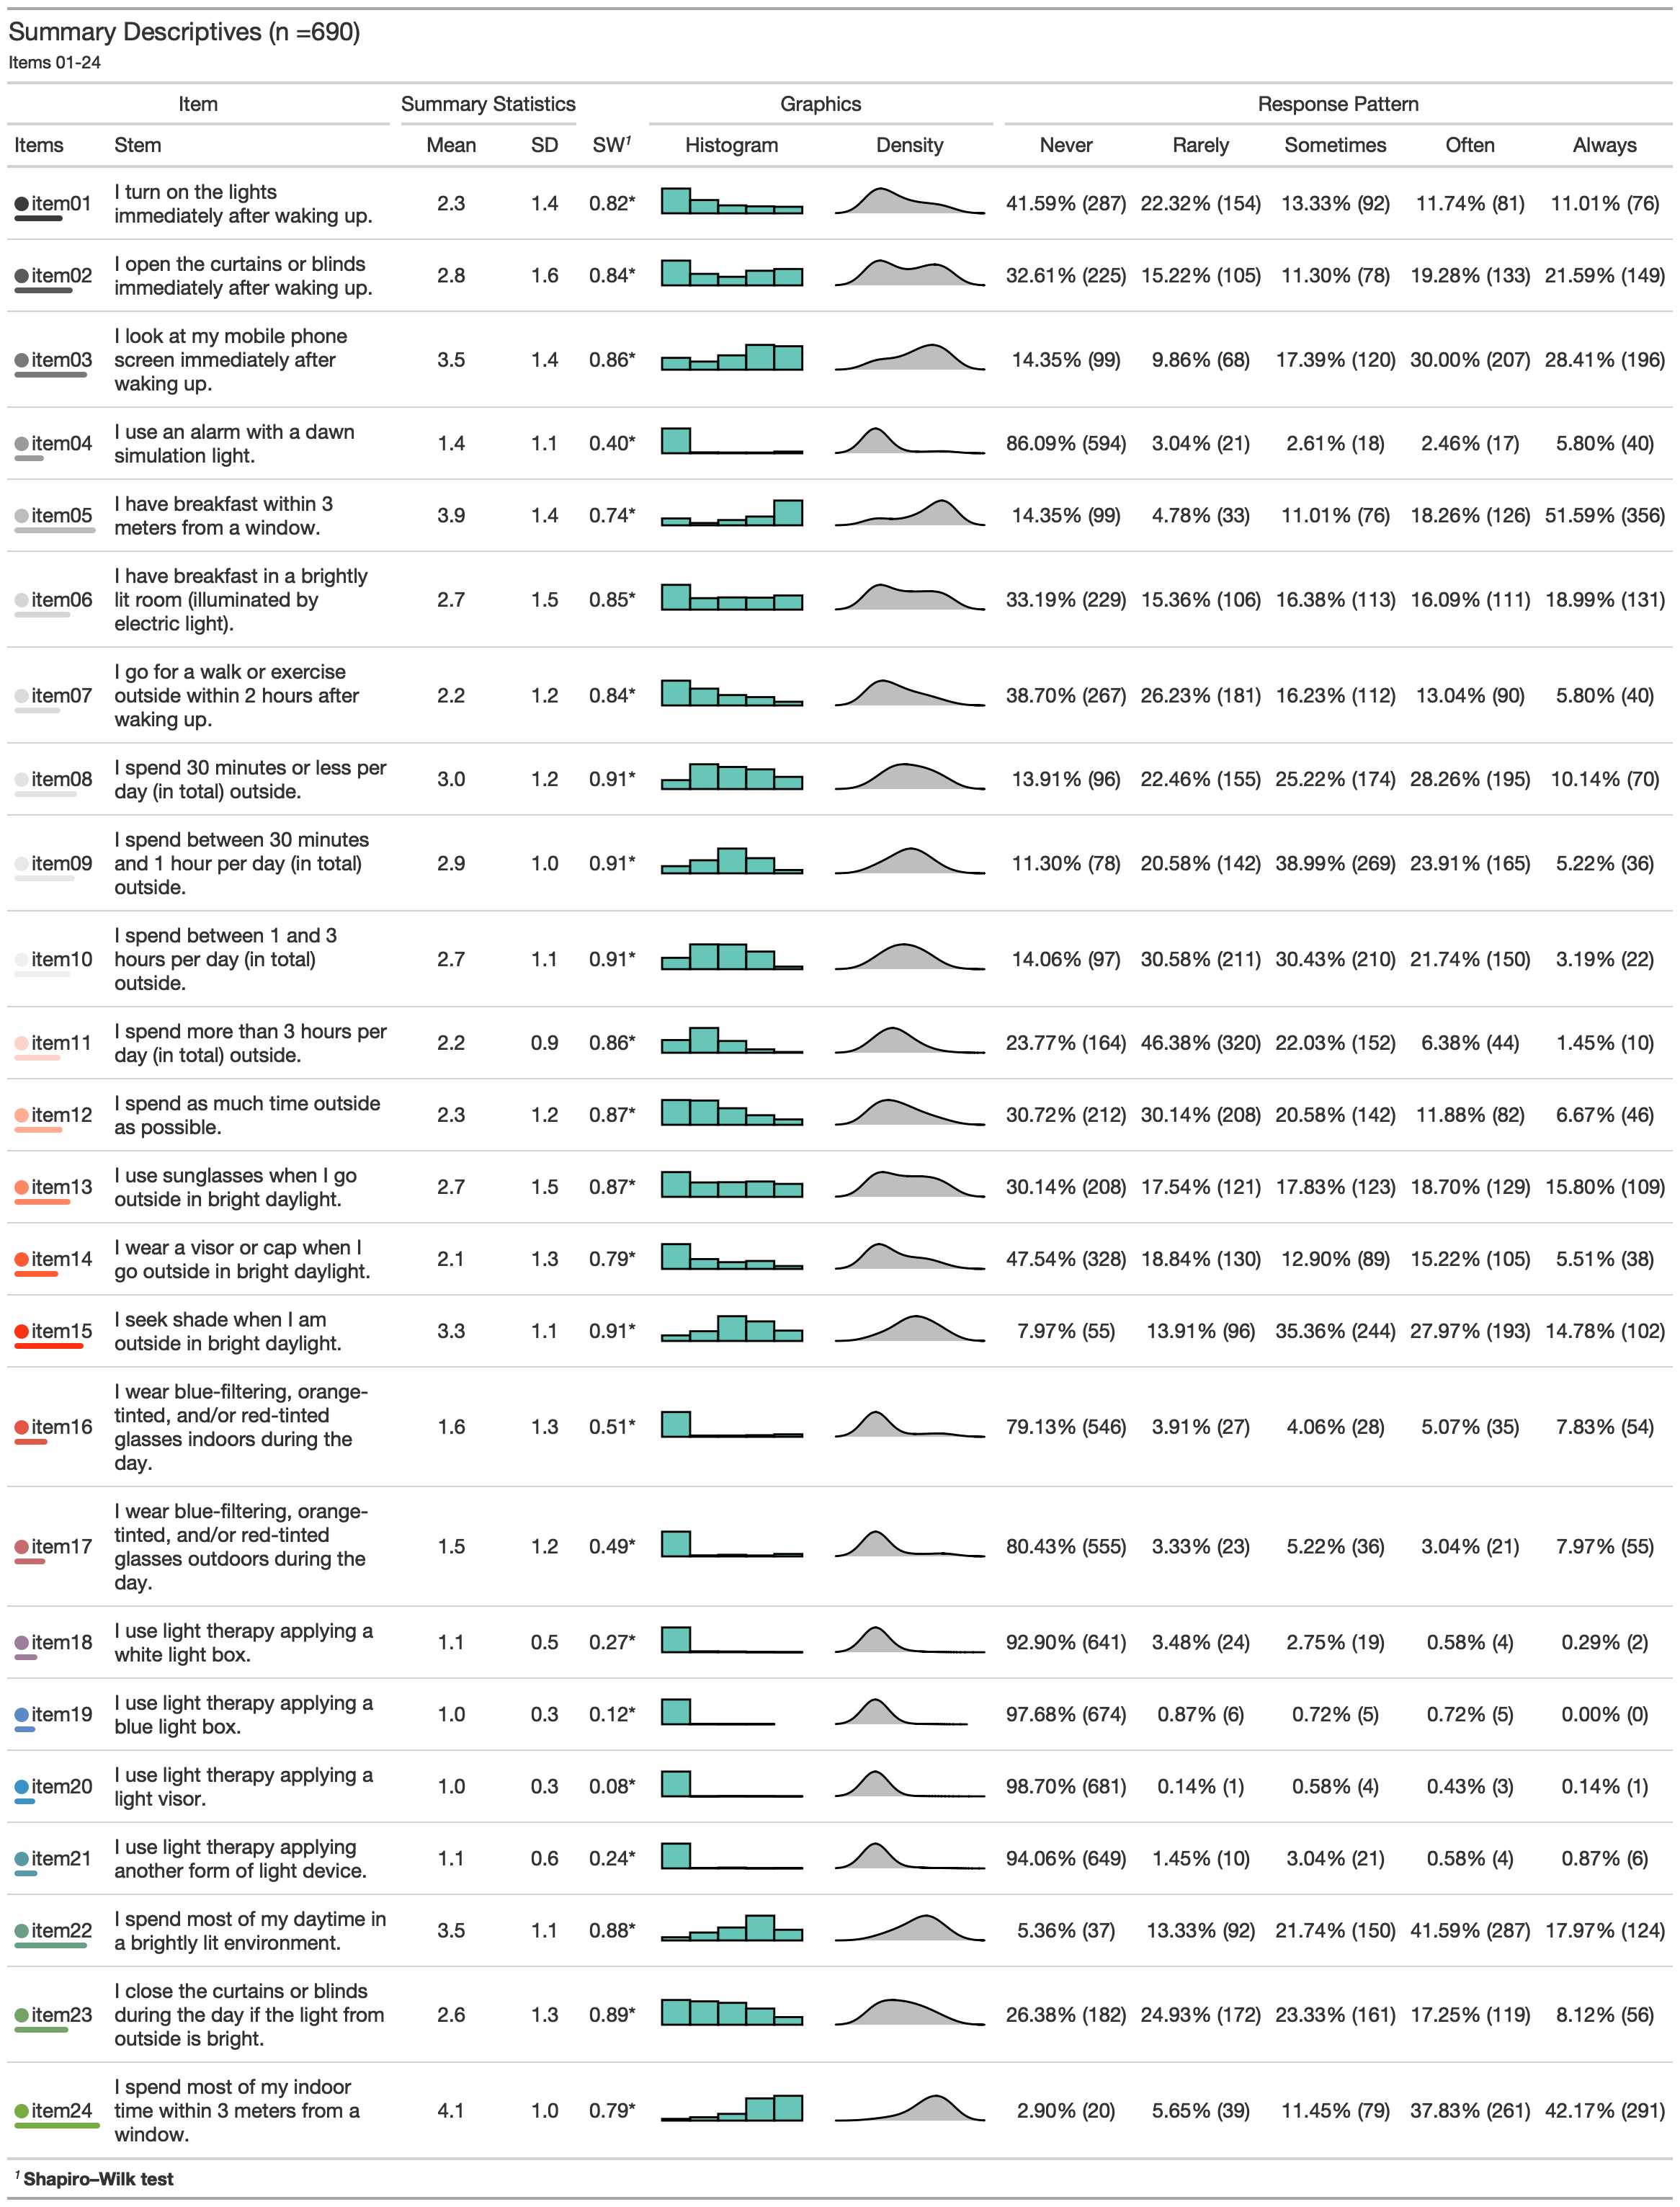
\includegraphics[width=2.5\linewidth,height=1\textheight]{Figures/Figure2} \caption{Summary descriptives and response pattern observed in the large-scale survey for item 01-24. All items violated normality assumption.}\label{fig:efagtPic1}
\end{figure}

\begin{figure}
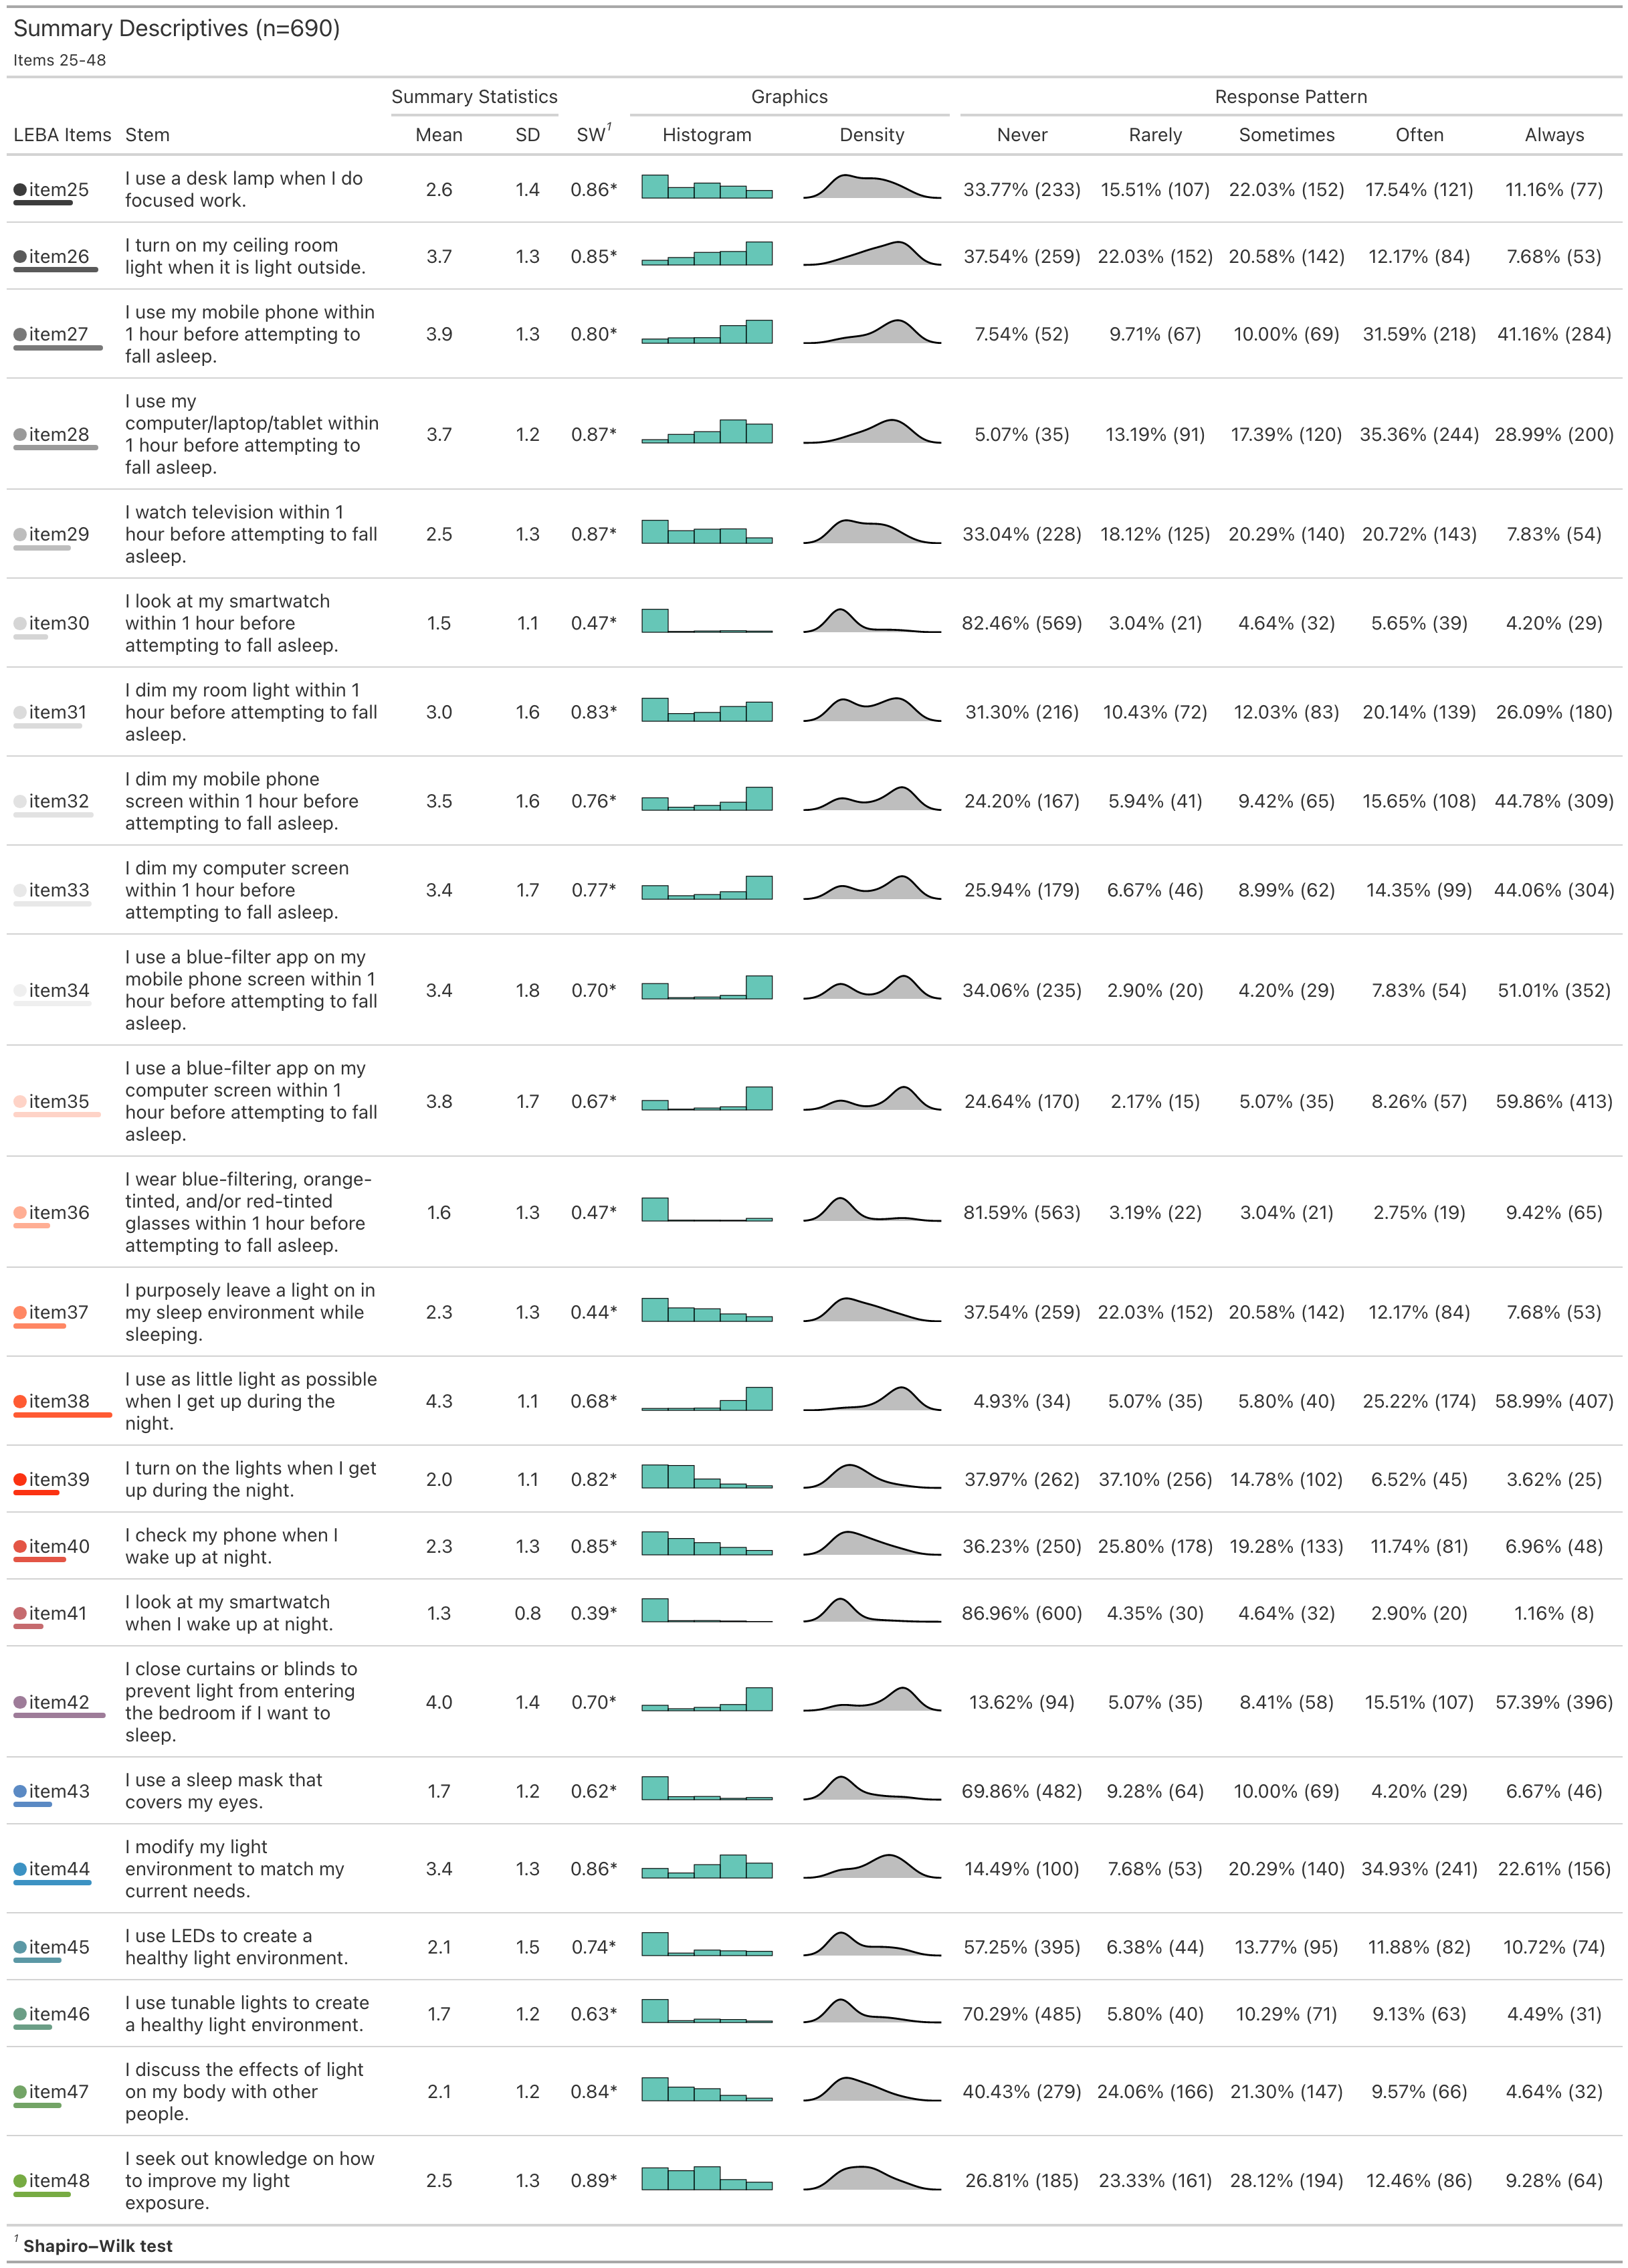
\includegraphics[width=2.5\linewidth,height=1\textheight]{Figures/Figure3} \caption{Summary descriptives and response pattern observed in the large-scale survey for item 25-48. All items violated normality assumption.}\label{fig:efagtPic2}
\end{figure}

We observed that the response patterns of LEBA inventory for the entire sample (n=690) were not normally distributed (Figures \ref{fig:efagtPic1} and \ref{fig:efagtPic2}). All items violated both univariate\textsuperscript{13} and multivariate normality\textsuperscript{14}. The multivariate skewness was 488.40 (p\textless0.001) and the multivariate kurtosis was 2,808.17 (p\textless0.001).

Similarly, non-normal distribution of response pattern was also observed in the EFA sample. \textbf{Supplementary Figure 1} depicts the univariate descriptive statistics for the EFA sample (n=428). Further, We observed that each item's correlation with the aggregated sum of the 48-item's score varied largely (corrected item-total correlation= 0.03 -0.48) indicating the possibility of multi-factor structure of the LEBA inventory.

\hypertarget{exploratory-factor-analysis-and-reliability-analysis}{%
\subsubsection{Exploratory factor analysis and reliability analysis}\label{exploratory-factor-analysis-and-reliability-analysis}}

Exploratory analysis revealed that items of LEBA inventory can be categorized into five major factors: (i) wearing blue light filters; (ii) spending time out doors; (iii) using phone and smartwatch in bed; (iv) using light before bedtime (v) using light in the morning and during daytime. In this stage of analysis, we retained 25 items. the first factor had three items and encapsulated the individual's preference for using blue light filters in different light environments. The second factor contained six items that incorporated the individuals' hours spent outdoors. The third factor contained five items that looked into specific behaviours of using a phone and smartwatch in bed. The fourth factor comprised five items investigated the other behaviours related to the individual's electric light exposure before bedtime. Lastly, the fifth factor encompassed six items capturing the individual's morning and daytime light exposure-related behaviour.

Prior to conducting the EFA, we have checked the post-hoc sampling adequacy by applying Kaiser-Meyer-Olkin (KMO) measures of sampling adequacy on the EFA sample (n=428)\textsuperscript{15} and the quality of the correlation matrix by Bartlett's test of sphericity\textsuperscript{16}. KMO\textgreater0.50 would indicate adequate sample size\textsuperscript{17} and a significant test of sphericity would indicate satisfactory quality of the correlation matrix . Results indicated that we had an adequate sample size (KMO=0.63) and correlation matrix (\(\chi^2_{1128}\)=5042.86, p\textless{} 0.001). However, 4.96\% of the inter-item correlation coefficients were greater than \textbar0.30\textbar, and the inter-item correlation coefficients ranged between -0.44 to 0.91. Figure \ref{fig:efa-plot-print}-A depicts the respective correlation matrix. To identify how many factors are required to optimally express human light exposure related behaviours we used a combination of methods. the Scree plot ( Figure \ref{fig:efa-plot-print}-B) revealed a six-factor solution, whereas the minimum average partial (MAP) method\textsuperscript{18} (\textbf{Supplementary Table 3}) and Hull method\textsuperscript{19} implied a five-factor solution (Figure \ref{fig:efa-plot-print}-C). Hence, we tested both five-factor and six-factor solutions using iterative EFA where we gradually identified and discarded problematic items (factor-loading \textless0.30 and cross-loading \textgreater0.30). In this process, we found a five-factor structure for LEBA inventory with 25 items. Table \ref{tab:EFATable} displays the factor-loading (\(\lambda\)) and communality of the items. Both factor loadings and commonalities advocate to accept this five-factor solution ( \textbar{}\(\lambda\)\textbar=0.32-0.99; commonalities=0.11-0.99). These five factors explains 10.25\%, 9.93\%, 8.83\%, 8.44\%, 6.14\% of the total variance in individual's light exposure related behaviours respectively. All factors exhibited excellent to satisfactory reliability (ordinal \(\alpha\)=0.94, 0.76, 0.75, 0.72, 0.62 respectively). The entire inventory also exhibited satisfactory reliability (\(\omega_t\)=0.77).

However, the histogram of the absolute values of nonredundant residual correlations (Figure \ref{fig:efa-plot-print}-D) displayed that 26\% of correlations were greater \textgreater\textbar.05\textbar, indicating a possible under-factoring.\textsuperscript{20}. Subsequently, we fitted a six-factor solution, where a factor with only two salient variables emerged, thus disqualifying the six-factor solution (\textbf{Supplementary Table 4}). While making the judgement of accepting this five-factor solution we considered both factor's interpretability and their psychometric properties. We deemed the five derived factors as highly interpretable and relevant concerning our aim to capture light exposure-related behaviour, we retained all of them with 25 items. Two of the items showed negative factor-loading (item 08: I spend 30 minutes or less per day (in total) outside. and item 37: I use a blue-filter app on my computer screen within 1 hour before attempting to fall asleep.). Upon re-inspection, we recognized these items to be negatively correlated to the respective factor, and thus, we reverse-scored these two items.



\begin{figure}

{\centering 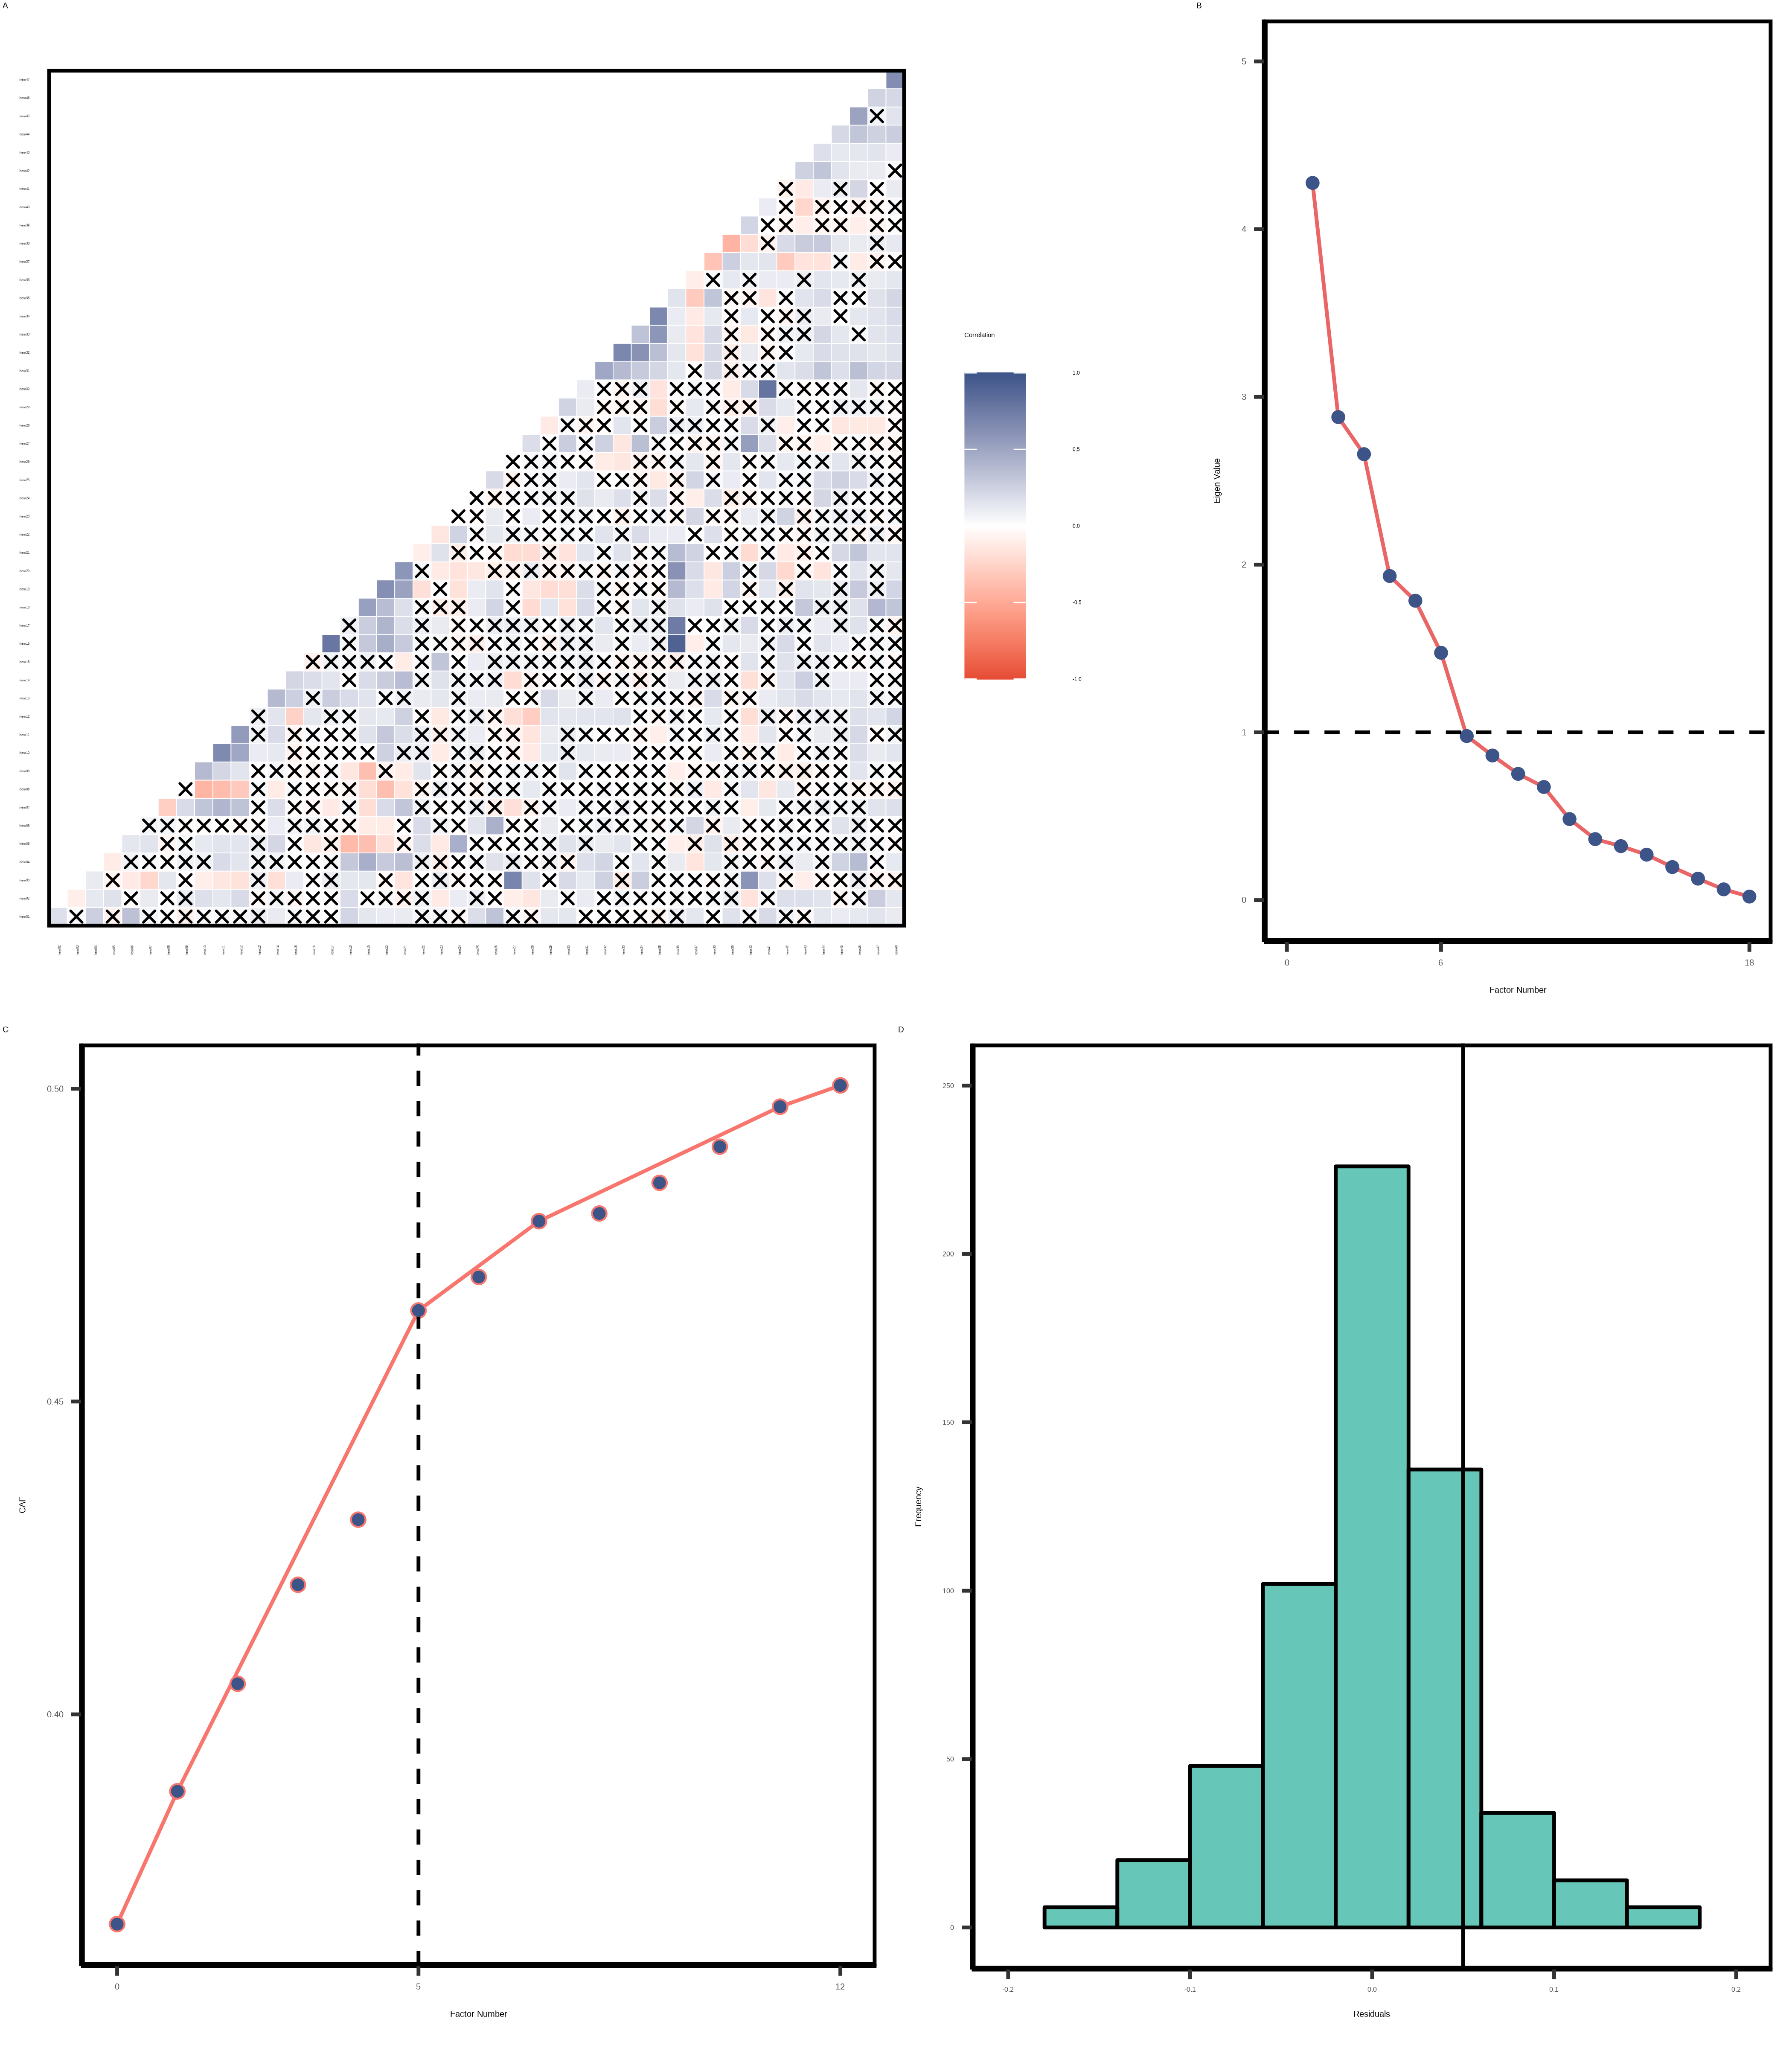
\includegraphics[width=1\linewidth,height=1.3\textheight]{Figures/Figure4} 

}

\caption{(A) Inter-item polychoric correlation coefficients for the 48 items. 4.9 \% inter-item correlation coefficients were higher than \textbar.30\textbar. `x' denotes non-significant correlation. (B) The Scree plot suggested six factors. (C) Hull method indicated that five factors were required to balance the model fit and number of parameters. (D) The histogram of nonredundant residual correlations in the five-factor model indicated that 26\% of inter-item correlations were higher than .05, hinting at a possible under-factoring.}\label{fig:efa-plot-print}
\end{figure}

\begin{lltable}

\begin{TableNotes}[para]
\normalsize{\textit{Note.} Only loading > .30 is reported.}
\end{TableNotes}

\footnotesize{

\begin{longtable}{p{1cm}p{10cm}p{1cm}p{1cm}p{1cm}p{1cm}p{1cm}p{1cm}}\noalign{\getlongtablewidth\global\LTcapwidth=\longtablewidth}
\caption{\label{tab:EFATable}Factor loadings and communality of the retained items in EFA using principal axis extraction method (n=482).}\\
\toprule
item & \multicolumn{1}{c}{Stem} & \multicolumn{1}{c}{PA1} & \multicolumn{1}{c}{PA2} & \multicolumn{1}{c}{PA3} & \multicolumn{1}{c}{PA4} & \multicolumn{1}{c}{PA5} & \multicolumn{1}{c}{Communality}\\
\midrule
\endfirsthead
\caption*{\normalfont{Table \ref{tab:EFATable} continued}}\\
\toprule
item & \multicolumn{1}{c}{Stem} & \multicolumn{1}{c}{PA1} & \multicolumn{1}{c}{PA2} & \multicolumn{1}{c}{PA3} & \multicolumn{1}{c}{PA4} & \multicolumn{1}{c}{PA5} & \multicolumn{1}{c}{Communality}\\
\midrule
\endhead
item16 & I wear blue-filtering, orange-tinted, and/or red-tinted glasses indoors during the day. & 0.99 &  &  &  &  & 0.99\\
item36 & I wear blue-filtering, orange-tinted, and/or red-tinted glasses within 1 hour before attempting to fall asleep. & 0.94 &  &  &  &  & 0.90\\
item17 & I wear blue-filtering, orange-tinted, and/or red-tinted glasses outdoors during the day. & 0.8 &  &  &  &  & 0.66\\
item11 & I spend more than 3 hours per day (in total) outside. &  & 0.79 &  &  &  & 0.64\\
item10 & I spend between 1 and 3 hours per day (in total) outside. &  & 0.76 &  &  &  & 0.59\\
item12 & I spend as much time outside as possible. &  & 0.65 &  &  &  & 0.47\\
item07 & I go for a walk or exercise outside within 2 hours after waking up. &  & 0.5 &  &  &  & 0.27\\
item08 & I spend 30 minutes or less per day (in total) outside. &  & -0.49 &  &  &  & 0.25\\
item09 & I spend between 30 minutes and 1 hour per day (in total) outside. &  & 0.32 &  &  &  & 0.11\\
item27 & I use my mobile phone within 1 hour before attempting to fall asleep. &  &  & 0.8 &  &  & 0.66\\
item03 & I look at my mobile phone screen immediately after waking up. &  &  & 0.8 &  &  & 0.68\\
item40 & I check my phone when I wake up at night. &  &  & 0.65 &  &  & 0.46\\
item30 & I look at my smartwatch within 1 hour before attempting to fall asleep. &  &  & 0.45 &  &  & 0.35\\
item41 & I look at my smartwatch when I wake up at night. &  &  & 0.36 &  &  & 0.33\\
item33 & I dim my computer screen within 1 hour before attempting to fall asleep. &  &  &  & 0.74 &  & 0.56\\
item32 & I dim my mobile phone screen within 1 hour before attempting to fall asleep. &  &  &  & 0.73 &  & 0.62\\
item35 & I use a blue-filter app on my computer screen within 1 hour before attempting to fall asleep. &  &  &  & 0.66 &  & 0.45\\
item37 & I purposely leave a light on in my sleep environment while sleeping. &  &  &  & -0.39 &  & 0.17\\
item38 & I use as little light as possible when I get up during the night. &  &  &  & 0.38 &  & 0.18\\
item46 & I use tunable lights to create a healthy light environment. &  &  &  &  & 0.6 & 0.42\\
item45 & I use LEDs to create a healthy light environment. &  &  &  &  & 0.59 & 0.37\\
item25 & I use a desk lamp when I do focused work. &  &  &  &  & 0.41 & 0.19\\
item04 & I use an alarm with a dawn simulation light. &  &  &  &  & 0.41 & 0.22\\
item01 & I turn on the lights immediately after waking up. &  &  &  &  & 0.4 & 0.17\\
item26 & I turn on my ceiling room light when it is light outside. &  &  &  &  & 0.35 & 0.16\\
% of Variance &  & 0.1 & 0.1 & 0.09 & 0.08 & 0.06 & NA\\
\bottomrule
\addlinespace
\insertTableNotes
\end{longtable}

}

\end{lltable}

\hypertarget{confirmatory-factor-analysis}{%
\subsubsection{Confirmatory factor analysis}\label{confirmatory-factor-analysis}}

To investigate the structural validity of the five-factor structure obtained in EFA, we conducted a confirmatory factor analysis (CFA) on the CFA sample. The five-factor structure with 25 items showed acceptable fit (Table \ref{tab:tabCfa}) providing evidence of structural validity (CFI=0.92; TLI=0.91; RMSEA=0.07 {[}0.06-0.07, 90\% CI{]}). Two equity constraints were imposed on item pairs 32-33 (item 32: I dim my mobile phone screen within 1 hour before attempting to fall asleep; item 33: I dim my computer screen within 1 hour before attempting to fall asleep) and 16-17 (item 16: I wear blue-filtering, orange-tinted, and/or red-tinted glasses indoors during the day; item 17: I wear blue-filtering, orange-tinted, and/or red-tinted glasses outdoors during the day). Item pair 32-33 describes the preference for dimming the electric devices' brightness before bedtime, whereas item pair 16-17 represents the use of blue filtering or coloured glasses during the daytime. Given the similar nature of captured behaviours within each item pair, we accepted the imposed equity constraints. Nevertheless, the SRMR value exceeded the guideline recommendation (SRMR=0.12). In order to improve the model fit, we conducted a post-hoc model modification. Firstly, the modification indices suggested cross-loadings between item 37 and 26 (item 37: I purposely leave a light on in my sleep environment while sleeping; item 26: I turn on my ceiling room light when it is light outside), which were hence discarded. Secondly, items 30 and 41 (item 30: I look at my smartwatch within 1 hour before attempting to fall asleep; item 41: I look at my smartwatch when I wake up at night) showed a tendency to co-vary in their error variance (MI=141.127, p\textless0.001 ). By allowing the latter pair of items (30 \(\&\) 41) to co-vary, the model's error variance attained an improved fit (CFI=0.95; TLI=0.95); RMSEA=0.06 {[}0.05-0.06, 90\% CI{]}; SRMR=0.11).

Accordingly, we accept the five-factor model with 23 items, finalizing the long Form of LEBA inventory (see \textbf{Supplementary File 1}). Internal consistency ordinal \(\alpha\) for the five factors of the LEBA were 0.96, 0.83, 0.70, 0.69, 0.52, respectively. The reliability of the total inventory was satisfactory (\(\omega_t\)=0.68). Figure \ref{fig:figcfa} depicts the obtained CFA structure, while \textbf{Supplementary Figure 2} depicts the data distribution and endorsement pattern of the retained 23 items in our CFA sample.

\begin{lltable}

\begin{TableNotes}[para]
\normalsize{\textit{Note.} df: Degrees of Freedom; CFI: Comparative Fit Index; TLI: Tucker Lewis Index; RMSEA: Root Mean Square Error of Approximation; CI: Confidence Interval; SRMR: Standardized Root Mean Square.}
\end{TableNotes}

\begin{longtable}{ccccccccc}\noalign{\getlongtablewidth\global\LTcapwidth=\longtablewidth}
\caption{\label{tab:tabCfa}Confirmatory Factor Analysis model fit indices of the two model: (a) Model 1: five factor model with 25 items (b) Model 2:  five factor model with 23 items. Model 2 attained the best fit.}\\
\toprule
Model & \multicolumn{1}{c}{$\chi^{2}$} & \multicolumn{1}{c}{df} & \multicolumn{1}{c}{CFI} & \multicolumn{1}{c}{TLI} & \multicolumn{1}{c}{RMSEA} & \multicolumn{1}{c}{RMSEA 90\% Lower CI} & \multicolumn{1}{c}{RMSEA 90\% Upper CI} & \multicolumn{1}{c}{SRMR}\\
\midrule
\endfirsthead
\caption*{\normalfont{Table \ref{tab:tabCfa} continued}}\\
\toprule
Model & \multicolumn{1}{c}{$\chi^{2}$} & \multicolumn{1}{c}{df} & \multicolumn{1}{c}{CFI} & \multicolumn{1}{c}{TLI} & \multicolumn{1}{c}{RMSEA} & \multicolumn{1}{c}{RMSEA 90\% Lower CI} & \multicolumn{1}{c}{RMSEA 90\% Upper CI} & \multicolumn{1}{c}{SRMR}\\
\midrule
\endhead
1 & 675.55 & 267.00 & 0.92 & 0.91 & 0.07 & 0.06 & 0.07 & 0.12\\
2 & 561.25 & 231.00 & 0.95 & 0.95 & 0.07 & 0.05 & 0.06 & 0.11\\
\bottomrule
\addlinespace
\insertTableNotes
\end{longtable}

\end{lltable}

\begin{figure}
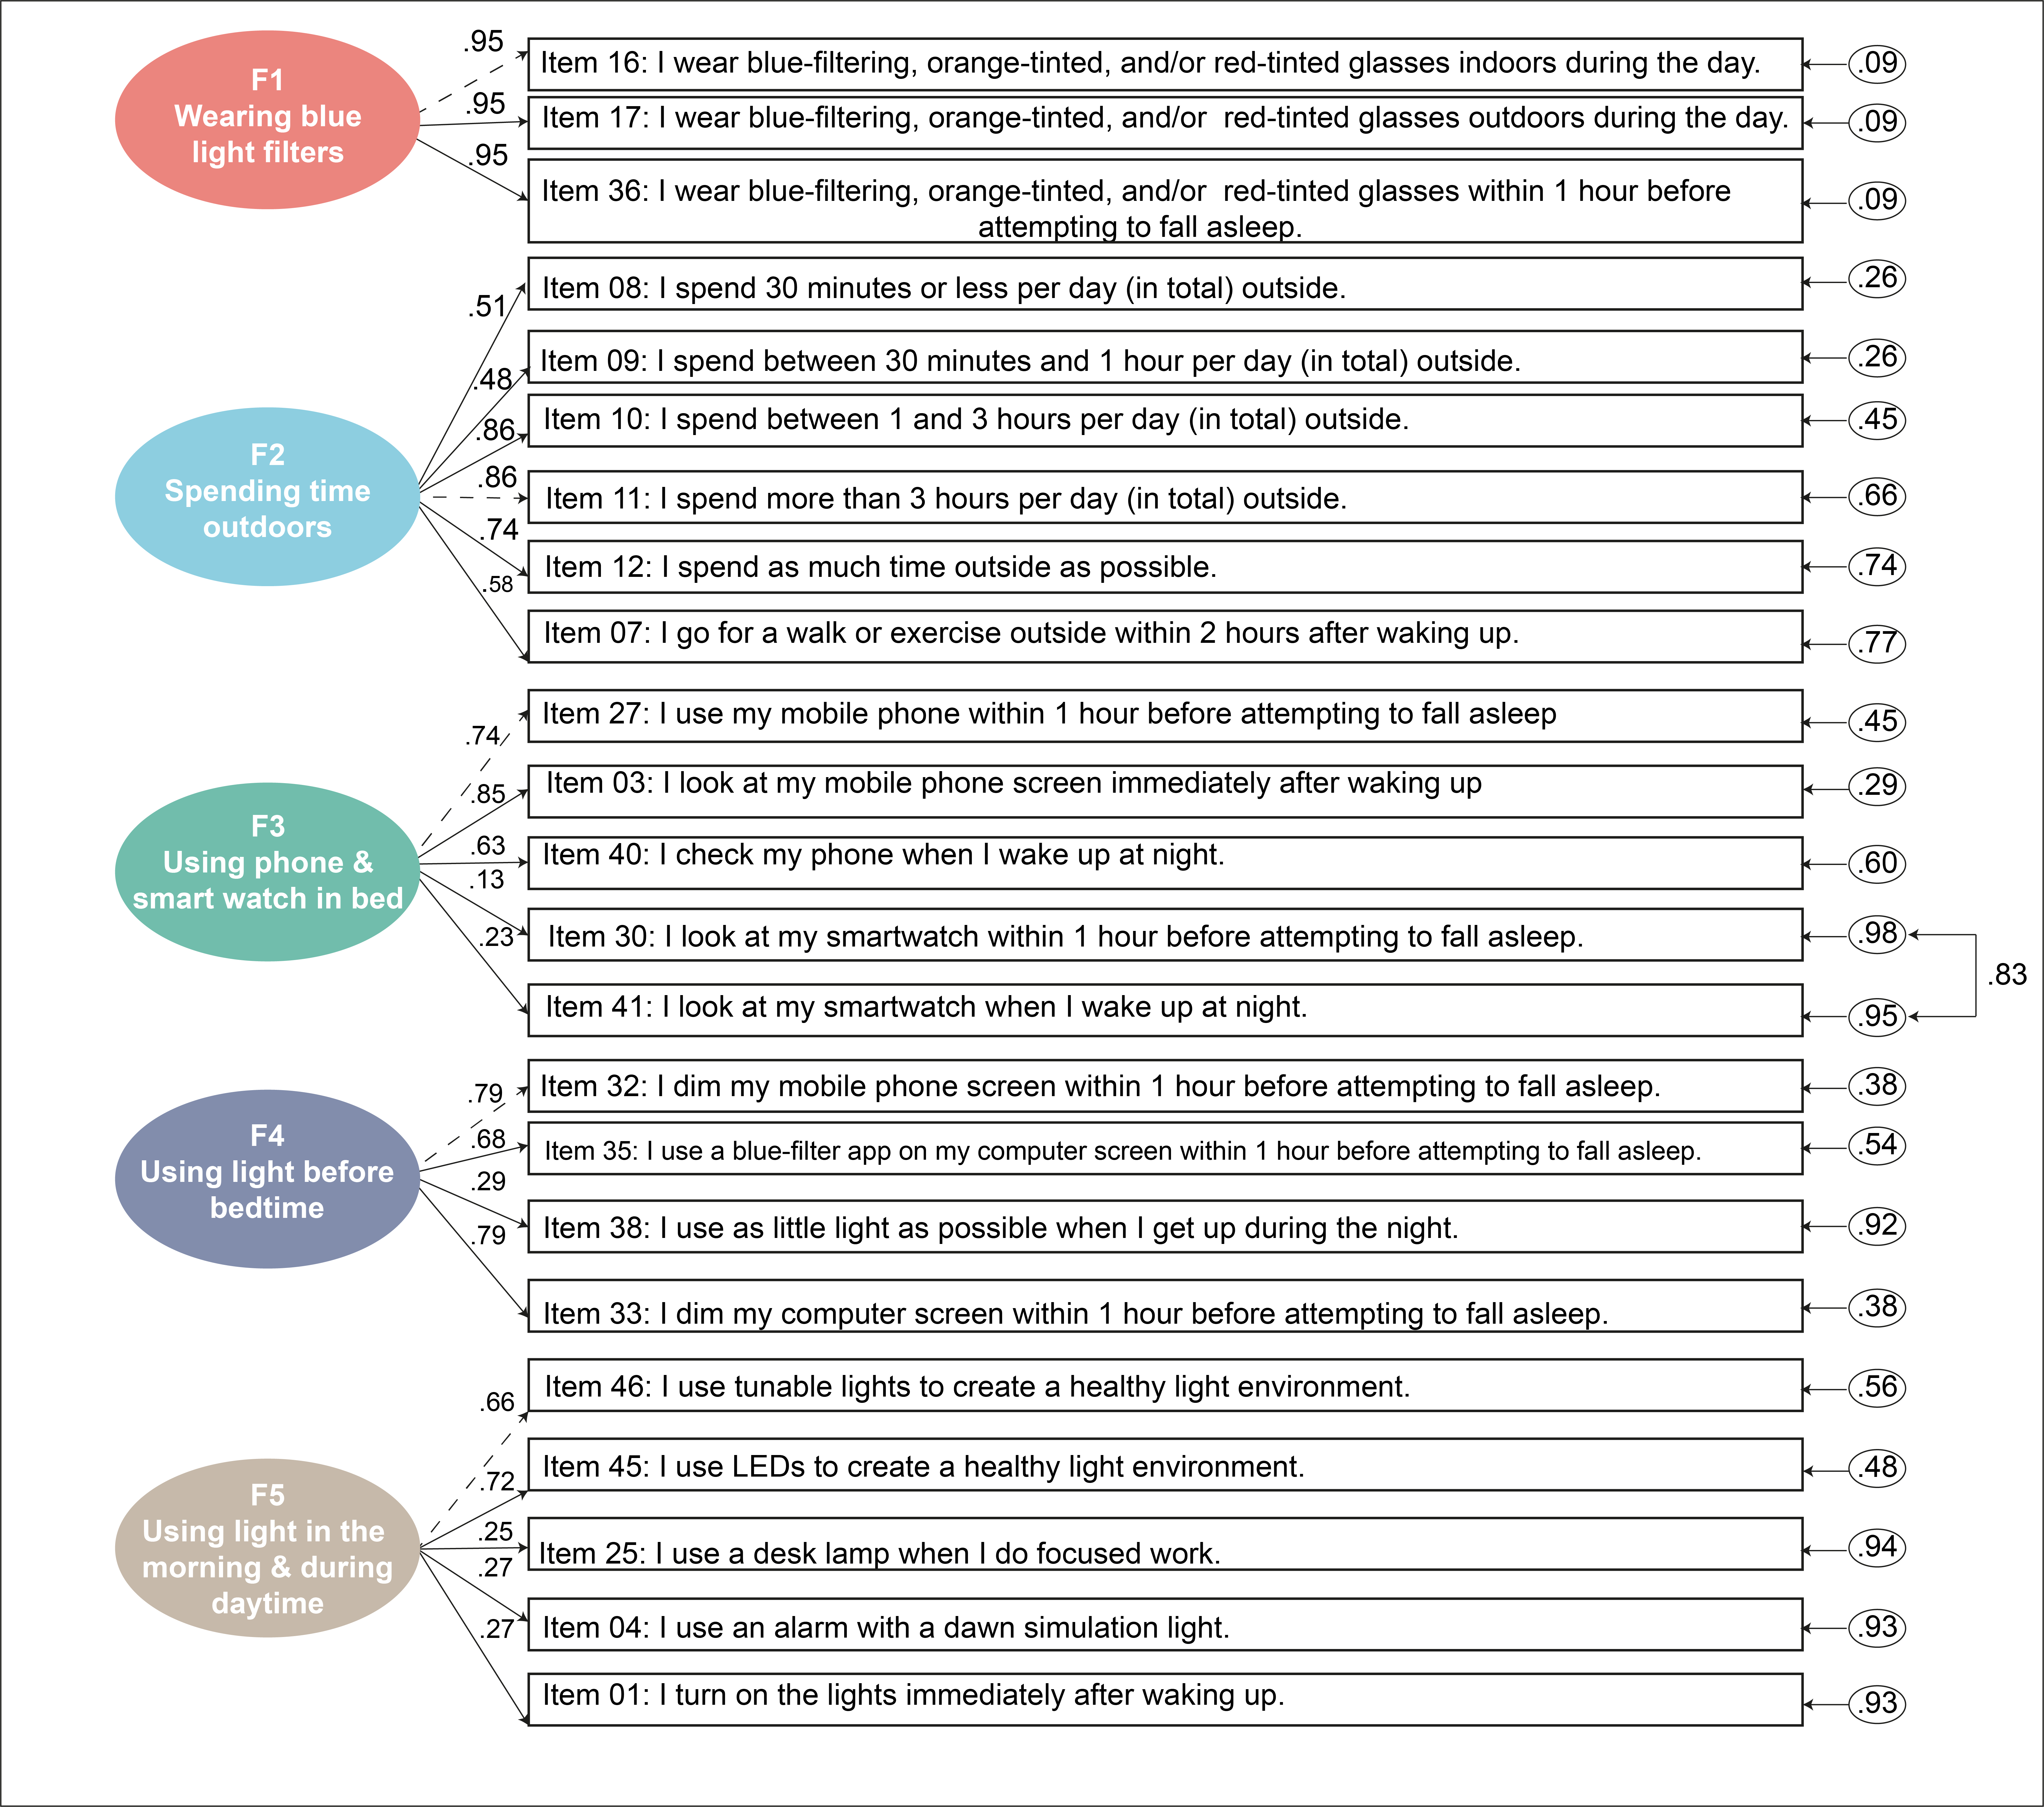
\includegraphics[width=1\linewidth,height=1\textheight]{Figures/Figure5} \caption{Five factor  model of LEBA obtained by confirmatory factor analysis. By allowing item pair 41 and 30 to co-vary their error variance our model attained the best fit.}\label{fig:figcfa}
\end{figure}

\hypertarget{measurement-invariance}{%
\subsubsection{Measurement invariance}\label{measurement-invariance}}

We reported the measurement invariance (MI) analysis on the CFA sample based on native (n=129) and non-native English speakers (n=133). A detailed demographic description are provided in \textbf{Supplementary Table 5}. Our MI results (Table \ref{tab:InvarianceTab}) indicated that LEBA inventory demonstrated highest level of (residual model) psychometric equivalence across native and non-native English speaking participants, thus permitting group-mean based comparisons. The four fitted MI models generated acceptable fit indices and the model fit did not significantly decrease across the nested models (\(\Delta\)CFI\textgreater-0.01; \(\Delta\)RMSEA\textless0.01).

\begin{lltable}

\begin{TableNotes}[para]
\normalsize{\textit{Note.} df: Degrees of Freedom; CFI: Comparative Fit Index; TLI: Tucker Lewis Index; RMSEA: Root Mean Square Error of Approximation; CI: Confidence Interval; SRMR: Standardized Root Mean Square; a=Metric vs Configural; b=Scalar vs Metric; c=Residual vs Scalar; *= df of model comparison.}
\end{TableNotes}

\footnotesize{

\begin{longtable}{ccccccccccc}\noalign{\getlongtablewidth\global\LTcapwidth=\longtablewidth}
\caption{\label{tab:InvarianceTab}Measurement Invariance analysis on CFA sample (n=262) across native and non-native English speakers.}\\
\toprule
 & \multicolumn{1}{c}{$\chi^{2}$} & \multicolumn{1}{c}{df} & \multicolumn{1}{c}{CFI} & \multicolumn{1}{c}{TLI} & \multicolumn{1}{c}{RMSEA} & \multicolumn{1}{c}{RMSEA 90\% Lower CI} & \multicolumn{1}{c}{RMSEA 90\% Upper} & \multicolumn{1}{c}{$\Delta$ $\chi^{2}$} & \multicolumn{1}{c}{$\Delta$ df*} & \multicolumn{1}{c}{p}\\
\midrule
\endfirsthead
\caption*{\normalfont{Table \ref{tab:InvarianceTab} continued}}\\
\toprule
 & \multicolumn{1}{c}{$\chi^{2}$} & \multicolumn{1}{c}{df} & \multicolumn{1}{c}{CFI} & \multicolumn{1}{c}{TLI} & \multicolumn{1}{c}{RMSEA} & \multicolumn{1}{c}{RMSEA 90\% Lower CI} & \multicolumn{1}{c}{RMSEA 90\% Upper} & \multicolumn{1}{c}{$\Delta$ $\chi^{2}$} & \multicolumn{1}{c}{$\Delta$ df*} & \multicolumn{1}{c}{p}\\
\midrule
\endhead
Configural & 632.20 & 442.00 & 0.95 & 0.94 & 0.06 & 0.05 & 0.07 & - & - & -\\
Metric & 643.06 & 458.00 & 0.95 & 0.95 & 0.06 & 0.04 & 0.07 & 18.254a & 16 & 0.309\\
Scalar & 711.87 & 522.00 & 0.95 & 0.95 & 0.05 & 0.04 & 0.06 & 68.221b & 64 & 0.336\\
Residual & 711.87 & 522.00 & 0.95 & 0.95 & 0.05 & 0.04 & 0.06 & 0c & 0 & NA\\
\bottomrule
\addlinespace
\insertTableNotes
\end{longtable}

}

\end{lltable}

\hypertarget{secondary-analysis-grade-level-identification-and-semantic-scale-network-analysis}{%
\subsection{Secondary analysis: Grade level identification and semantic scale network analysis}\label{secondary-analysis-grade-level-identification-and-semantic-scale-network-analysis}}

We investigated the language-based accessibility of LEBA using Flesch-Kincaid grade level analysis\textsuperscript{21}. Results indicated that at least a language proficiency of educational grade level-four (US education system) with age above eight years are required to comprehend the items used in LEBA inventory. Semantic Scale analysis\textsuperscript{22} was administered to assess the LEBA's (23 items) semantic relation to other questionnaires. LEBA inventory was most strongly semantically related to scales about sleep: The ``Sleep Disturbance Scale For Children''\textsuperscript{23} and the ``Composite International Diagnostic Interview (CIDI): Insomnia''\textsuperscript{24}. The cosine similarity index ranged between 0.47 to 0.51.

\hypertarget{developing-a-short-form-of-leba-irt-based-analysis}{%
\subsection{Developing a short form of LEBA: IRT-based analysis}\label{developing-a-short-form-of-leba-irt-based-analysis}}

Our aim was to provide a data-driven approach to reducing the number of items for cases where a small reduction of items is necessary. In order to derive a short form of the LEBA inventory, we fitted each factor of the LEBA with the graded response model\textsuperscript{25} to the combined EFA and CFA sample (n=690). The resulting item discrimination parameters of the inventory fell into categories of ``very high'' (10 items), ``high'' (4 items), ``moderate'' (4 items), and ``low'' ( 5 items), indicating a good range of discrimination along the latent trait level (\(\theta\)) (\textbf{Supplementary Table 6}). An examination of the item information curve (\textbf{Supplementary Figure 3}) revealed five items (1, 25, 30, 38, \& 41) provided very low information regarding light exposure related behaviours with relatively flat curves (I(\(\theta\)) \textless0.20). We discarded those items, culminating in a short form of LEBA with five factors and 18 items (\textbf{Supplementary File 2}).

\begin{figure}
\includegraphics[width=1\linewidth,height=1.2\textheight]{Figures/Figure6} \caption{Test information curves for the five factors of LEBA: (A) wearing blue light filters (B) spending time outdoors (C) using a phone and smartwatch in bed (D) using light before bedtime (E) using light in the morning and during daytime. Along the x-axis, we plotted the underlying latent trait continuum for each factor. Along the y-axis, we plotted how much information a particular factor is carrying across its latent trait continuum}\label{fig:Testinfo}
\end{figure}

Subsequently, we obtained five test information curves (TICs). As Figure \ref{fig:Testinfo} illustrates, the TICs of the first and fifth factors peaked on the right side of the centre of their latent traits, while the TICs of the other three factors were roughly centred on the respective trait continuum (\(\theta\)). This points out that the LEBA short-form estimates the light exposure-related behaviour most precisely near the centre of the trait continuum for the second, third and fourth factors. In contrast, for the first and fifth factors the TICs were left skewed indicating their increased sensitivity in identifying people who are engaging more in those particular light exposure related behaviour dimensions\textsuperscript{26}.

Finally, \textbf{Supplementary Table 7} summarises the item fit indexes of the LEBA short form. All 18 items yielded RMSEA value \(\le\) 0.06, indicating an adequate fit to the fitted IRT model. Furthermore, \textbf{Supplementary Figure 4} depicts the person fit Zh statistics histogram for the five IRT models. Zh statistics are larger than -2 for most participants, suggesting a good person fit regarding the selected IRT models.

\hypertarget{discussion}{%
\section{Discussion}\label{discussion}}

We have developed two versions of a self-report inventory, LEBA, that can capture light exposure-related behaviours in multiple dimensions. The 48 generated items were applied in a large-scale, geographically unconstrained, cross-sectional study, yielding 690 completed surveys. To assure high data quality, participant responses were only included when the five ``attention check items'' throughout the survey were passed. Ultimately, data was recorded from 74 countries and 28 time zones, including native and non-native English speakers from a sex-balanced and age-diverse sample (see Table 1). The acquired study population complied with our objective to avoid bias from a selective sample, which is crucial when relying on voluntary uncompensated participation.

Data collected in the first round was used to explore the latent structure (EFA sample; n=428). The exploratory factor analysis revealed a highly interpretable five-factor solution (``Wearing blue light filters'', ``Spending time outdoors'', ``Using phone and smartwatch in bed'', ``Using light before bedtime'', and ``Using light in the morning and during daytime'') with 25 items. Our CFA analysis (CFA sample; n=262) confirmed the five-factor structure we obtained in our EFA, thus providing evidence for structural validity.(CFI=0.95; TLI=0.95; RMSEA=0.06). In this model, we discarded two more items (item 26 \(\&\) 37 ) for possible cross-loadings. As a rule of thumb, reliability coefficients higher than .70 are regarded as ``satisfactory''. However, at the early developmental stage, a value of .50 is considered acceptable\textsuperscript{27--29}. Thus, we confer, the internal consistency coefficients ordinal alpha for the five factors and the total inventory were satisfactory (Ordinal alpha ranged between 0.52 to 0.96; McDonald's \(\omega_t\)=0.68).

The results of the measurement invariance analysis indicate that the construct ``Light exposure-related behaviour'' is equivalent across native and non-native English speakers and thus suitable for assessment in both groups. Furthermore, according to the grade level identification method, the LEBA appears understandable for students at least 8.33 years of age visiting grade four or higher. Interestingly, the semantic similarity analysis (``Semantic Scale Network'' database\textsuperscript{22}) revealed that the ``LEBA'' is semantically related to the ``Sleep Disturbance Scale For Children'' (SDSC)\textsuperscript{23} and the ``Composite International Diagnostic Interview (CIDI): Insomnia''\textsuperscript{24}. Upon inspecting the questionnaire contents, we found that some items in the factors ``Using phone and smartwatch in bed'' and ``Using light before bedtime'' have semantic overlap with the SDSC's and CIDI's items. However, while the CIDI and the SDSC capture various clinically relevant sleep problems and related activities, the LEBA aims to assess light-exposure-related behaviour. Since light exposure at night has been shown to influence sleep negatively\textsuperscript{7,30}, this overlap confirms our aim to measure the physiologically relevant aspects of light-exposure-related behaviour. Nevertheless, the general objectives of the complete questionnaires and the LEBA differ evidently.

While developing and validating LEBA, we have complemented conventional approaches with an Item Response Theory (IRT) analysis. IRT provides a framework to interpret respondents' obtained scores in the light of latent ability (i.e.~light exposure behaviour) and the characteristics of the respondents -- how they interpret the items\textsuperscript{31}. The benefit of implementing IRT analysis was twofold. First, we derived a shorter form of LEBA (18 items). We fitted a graded response model to the combined EFA and CFA sample (n=690) and discarded five items (1, 25, 30, 38, \& 41) with relatively flat item information curve {[}I(\(\theta\)) \textless.20{]}. The resulting test information curves suggest that the short-LEBA is a psychometrically sound measure with adequate coverage of underlying traits and can be applied to capture the frequency of different light exposure related behaviours reliably. Often, psychological measurements require application of several questionnaires simultaneously. Responding to several lengthy questionnaires increases the participants losing focus and becoming tired. Thus, in some circumstances, reducing the number of items even slightly may be necessary to employ the LEBA questionnaire. Our aim was to provide a data-driven approach to reducing the number of items, apart from the possibility of excluding a specific factor from the 23-item questionnaire. Nonetheless, where possible, we strongly recommend using the extended form of the questionnaire to avoid limiting the range of gained information.

The IRT analysis enabled us to capture individual differences in responding to the items of LEBA. Findings from the item and person fit index analysis demonstrate that all five fitted models were acceptable and provide evidence of validity for the factors. In addition, the diverse item discrimination parameters indicate an appropriate range of discrimination -- the ability to differentiate respondents with different levels of light exposure-related behaviour while acknowledging the interpersonal variability in understanding the item.

\hypertarget{known-limitations}{%
\subsection{Known limitations}\label{known-limitations}}

We acknowledge that this work is limited concerning the following aspects:

The fifth factor, ``using light in the morning and during daytime'', exhibited low internal consistency both in the exploratory and confirmatory factor analysis (EFA: 0.62; CFA:0.52 ). Since, it was above .50, considering the developmental phase of this inventory we accepted the fifth factor. This particular factor captures our behaviour related to usages of light in the morning and daytime. Since, light exposure during morning and daytime influences our alertness and cognition\textsuperscript{32,33}, we deemed capturing these behaviours is essential for the sake of completeness of our inventory. However, the possibility of improving the reliability should be investigated further by adding more appropriate and relevant items to this factor.

The habitual patterns queried in the developed inventory might not exhaustively represent all relevant light-exposure-related behaviours. For instance, it is conceivable that additional light-related activities not included in the LEBA depend on the respondents' profession/occupation, geographical context, and socio-economic status. However, we generated the initial item pool with an international team of researchers and followed a thorough psychometric analysis. Therefore, we are confident that the developed LEBA inventory can serve as a good starting point for exploring the light exposure related behaviours in more depth and inform room for modification of light exposure-related behaviour to improve light hygiene.

As with all studies relying on retrospective self-report data, individuals filling in the LEBA may have difficulties precisely recalling the inquired light-related behaviours. In the interest of bypassing a substantial memory component, we limited the recall period to four weeks and chose response options that do not require exact memory recall. In contrast to directly assessing light properties via self-report, we assume that reporting behaviours might be more manageable for inexperienced laypeople, as the latter does not rely on existing knowledge about light sources. The comprehensibility of the LEBA is also reflected by the Flesch-Kincaid grade level identification method\textsuperscript{21} that suggested a minimum age of 8.33 years and an educational grade of four or higher (US grading system). We argue that measuring light-related behaviours via self-report is crucial because these behaviours will hardly be as observable by anyone else or measurable with other methods (like behavioural observations) with reasonable effort.

It is important to note that LEBA utilizes a five-point Likert-type response scale which may be susceptible to central tendency bias, i.e.~responses are biased towards the central value of the response scale. Future work should evaluate other methods of obtaining responses, such as using a visual-analogue scale.

Finally, there is limited evidence for convergent validity. LEBA being the first of its kind in characterising light exposure \emph{behaviour} at present lacks a gold standard against which its convergent validity evidence could be established. A recent study\textsuperscript{34} demonstrated the predictive validity of LEBA by successfully relating its factors to self-reported chronotype, mood, sleep quality, and cognitive function. The results of their study confirmed that light-related behaviours, as captured by LEBA, could led to different light exposure experiences that differentially influence health, wellness and performance. Further work will need to establish convergent validity of LEBA further.

\hypertarget{future-directions}{%
\subsection{Future directions}\label{future-directions}}

To our knowledge, the LEBA is the first inventory characterising light exposure-related behaviour in a scalable manner. Further evidence for the validity of the LEBA could be obtained by administering it conjointly with objective field measurements of light exposure (e.g.~with portable light loggers/wearables), smartphone readouts, as well as subjective data in the form of 24-hour recalls. Such a study could related the relationship bewteen (subjectively measured) light exposure-related behavioural patterns translate into (objectively measured) received light exposure, smartphone use, and how closely the retrospective questionnaire relates to daily reports of these behaviours.

\hypertarget{conclusion}{%
\subsection{Conclusion}\label{conclusion}}

Here, we developed a novel, internally consistent and structurally valid 23-item self-report inventory for capturing light exposure-related behaviour in five scalable factors. In addition, an 18-item short-form of the LEBA was derived using IRT analysis, yielding adequate coverage across the underlying trait continuum. Applying the LEBA inventory can provide insights into light exposure-related habits on a population-based level. Furthermore, it can serve as a good starting point to profile individuals based on their light exposure-related behaviour and to asseses their light consumption and timing.

\hypertarget{methods}{%
\section{Methods}\label{methods}}

\hypertarget{data-collection}{%
\subsection{Data collection}\label{data-collection}}

A quantitative cross-sectional, fully anonymous, geographically unconstrained online survey was conducted via REDCap\textsuperscript{35,36} by way of the University of Basel \href{https://redcap.scicore.unibas.ch}{sciCORE}. Participants were recruited via the \href{https://enlightenyourclock.org/participate-in-research}{website} (\url{https://enlightenyourclock.org/participate-in-research}) of the science-communication comic book ``Enlighten your clock'', co-released with the survey\textsuperscript{37}, social media (i.e., LinkedIn, Twitter, Facebook), mailing lists, word of mouth, the investigators' personal contacts, and supported by the distribution of the survey link via f.lux\textsuperscript{38}. The initial page of the online survey provided information about the study, including that participation was voluntary and that respondents could withdraw from participation at any time without being penalised. Subsequently, consent was recorded digitally for the adult participants (\textgreater18 years), while under-aged participants (\textless18 years) were prompted to obtain additional assent from their parents/legal guardians. Filling in all questionnaires was estimated to take less than 30 minutes, and participation was not compensated.

As a part of the demographic data, participants provided information regarding age, sex, gender identity, occupational status, COVID-19-related occupational setting, time zone/country of residence and native language. The demographic characteristics of our sample are given in \textbf{Table 1}. Participants were further asked to confirm that they participated in the survey for the first time. All questions incorporating retrospective recall were aligned to a ``past four weeks'' period. Additionally, four attention check items were included among the questionnaires to ensure high data quality, with the following phrasing:
- We want to make sure you are paying attention. What is 4+5?
- {[}\ldots{]} Please select ``Strongly disagree'' here.
- {[}\ldots{]} Please type in ``nineteen'' as a number.
- {[}\ldots{]} Please select ``Does not apply/I don't know.'' here.

\hypertarget{analytic-strategy}{%
\subsection{Analytic strategy}\label{analytic-strategy}}

Figure \ref{fig:FlowchartFig} summarises the steps we followed while developing the LEBA. We conducted all analyses with the statistical software environment R.

\begin{enumerate}
\def\labelenumi{(\arabic{enumi})}
\item
  We set an item pool of 48 items with a six-point Likert-type response format (0-Does not apply/I don't know, 1-Never, 2-Rarely 3-Sometimes, 4-Often, 5-Always) for our initial inventory. Our purpose was to capture light exposure-related behaviour. In that context, the first two response options: ``Does not apply/I don't know'' and ``Never'', provided similar information. As such, we collapsed them into one, making it a 5-point Likert-type response format (1-Never, 2-Rarely, 3-Sometimes, 4-Often, 5-Always).
\item
  Two rounds of data collection were administered. In the first round (EFA sample; n=428) we collected data for the exploratory factor analysis (EFA). A sample of at least 250-300 is recommended for EFA\textsuperscript{39,40}. The EFA sample exceeded this recommendation. The second round data (CFA sample; n=262) was subjected to confirmatory factor analysis (CFA). To assess sampling adequacy for CFA, we followed the N:q rule\textsuperscript{41--44}, where at least ten participants per item are required to earn trustworthiness of the result. Again, our CFA sample exceeded this guidelines.
\item
  We conducted descriptive and item analyses and proceeded to EFA on the EFA sample. Prior to the EFA, the necessary assumptions, including sample adequacy, normality assumptions, and quality of correlation matrix, were assessed. As our data violated both the univariate and multivariate normality assumption and yielded ordinal response data, we used a polychoric correlation matrix in the EFA and employed ``principal axis'' (PA) as the factor extraction method\textsuperscript{20,45}. We applied a combination of methods, including a Scree plot\textsuperscript{46}, minimum average partials method\textsuperscript{18}, and Hull method\textsuperscript{19} to identify factor numbers. To determine the latent structure, we followed the common guidelines: (i) no factors with fewer than three items (ii) no factors with a factor loading \textless0.3 (iii) no items with cross-loading \textgreater{} .3 across factors\textsuperscript{47}.
\end{enumerate}

Though Cronbach's internal consistency coefficient alpha is widely used for estimating internal consistency, it tends to deflate the estimates for Likert-type data since the calculation is based on the Pearson-correlation matrix, which requires response data to be continuous in nature\textsuperscript{48,49}. Subsequently, we reported ordinal alpha for each factor obtained in the EFA which was suggested as a better reliability estimates for ordinal data\textsuperscript{49}. We also estimated the internal consistency reliability of the total inventory using McDonald's \(\omega_t\) coefficient, which was suggested as a better reliability estimate for multidimensional constructs\textsuperscript{50,51}. Both ordinal alpha and McDonald's \(\omega_t\) coefficient values range between 0 to 1, where higher values represent better reliability.

To validate the latent structure obtained in the EFA, we conducted a categorical confirmatory factor analysis (CFA) with the weighted least squares means and variance adjusted (WLSMV) estimation\textsuperscript{20} on the CFA sample. We assessed the model fit using standard model fit guidelines: (i) \(\chi^2\) test statistics: a non-significant test statistics is required to accept the model (ii) comparative fit index (CFI) and Tucker Lewis index (TLI): close to 0.95 or above/ between 0.90-0.95 and above (iii) root mean square error of approximation (RMSEA): close to 0.06 or below, (iv) Standardized root mean square (SRMR): close to 0.08 or below\textsuperscript{52,53}. However, the \(\chi^2\) test is sensitive to sample size\textsuperscript{54}, and SRMR does not work well with ordinal data\textsuperscript{55}. Consequently, we judged the model fit using CFI, TLI and RMSEA.

In order to evaluate whether the construct demonstrated psychometric equivalence and the same meaning across native English speakers (n=129) and non-native English speakers (n=133) in the CFA sample (n=262)\textsuperscript{43,56} measurement invariance analysis was used. We used structural equation modelling framework to assess the measurement invariance. We successively compared four nested models: configural, metric, scalar, and residual models using the \(\chi^2\) difference test (\(\Delta \chi^2\)). Among MI models, the configural model is the least restrictive, and the residual model is the most restrictive. A non-significant \(\Delta \chi^2\) test between two nested measurement invariance models indicates mode fit does not significantly decrease for the superior model, thus allowing the superior invariance model to be accepted\textsuperscript{57,58}.

\begin{enumerate}
\def\labelenumi{(\arabic{enumi})}
\setcounter{enumi}{3}
\item
  In a secondary analysis, we identified the educational grade level (US education system) required to understand the items in our inventory with the Flesch-Kincaid grade level identification method\textsuperscript{21}. Correspondingly, we analysed possible semantic overlap of our developed inventory using the \href{https://rosenbusch.shinyapps.io/semantic_net/}{``Semantic Scale Network'' (SSN)} engine\textsuperscript{22}. The SSN detects semantically related scales and provides a cosine similarity index ranging between -.66 to 1\textsuperscript{22}. Pairs of scales with a cosine similarity index value of 1 inidicate full semantical similarity, suggesting redundancy.
\item
  We derived a short form of the LEBA employing an Item Response Theory (IRT) based analysis. We fitted each factor of the LEBA to the combined EFA and CFA sample (n=690) using the graded response model\textsuperscript{25}. IRT assesses the item quality by estimating the item discrimination, item difficulty, item information curve, and test information curve\textsuperscript{26}. Item discrimination indicates how well a particular item can differentiate between participants across the given latent trait continuum (\(\theta\)). Item difficulty corresponds to the latent trait level at which the probability of endorsing a particular response option is 50\%. The item information curve (IIC) indicates the amount of information an item carries along the latent trait continuum. Here, we reported the item difficulty and discrimination parameter and categorized the items based on their item discrimination index: (i) none=0; (ii) very low=0.01 to 0.34; (iii) low=0.35 to 0.64; (iv) moderate=0.65 to 1.34 ; (v) high=1.35 to 1.69; (vi) very high \textgreater1.70\textsuperscript{26}. We discarded the items with a relatively flat item information curve (information \textless.2) to derive the short form of LEBA. We also assessed the precision of the short LEBA utilizing the test information curve (TIC). TIC indicates the amount of information a particular scale carries along the latent trait continuum. Additionally, the item and person fit of the fitted IRT models were analysed to gather more evidence on the validity and meaningfulness of our scale\textsuperscript{20}. The item fit was evaluated using the RMSEA value obtained from Signed-\(\chi^2\) index implementation, where an RMSEA value \(\le\).06 was considered an adequate item fit. The person fit was estimated employing the standardized fit index Zh statistics\textsuperscript{59}. Here, Zh \textless{} -2 was considered as a misfit\textsuperscript{59}.
\end{enumerate}

\begin{figure}

{\centering 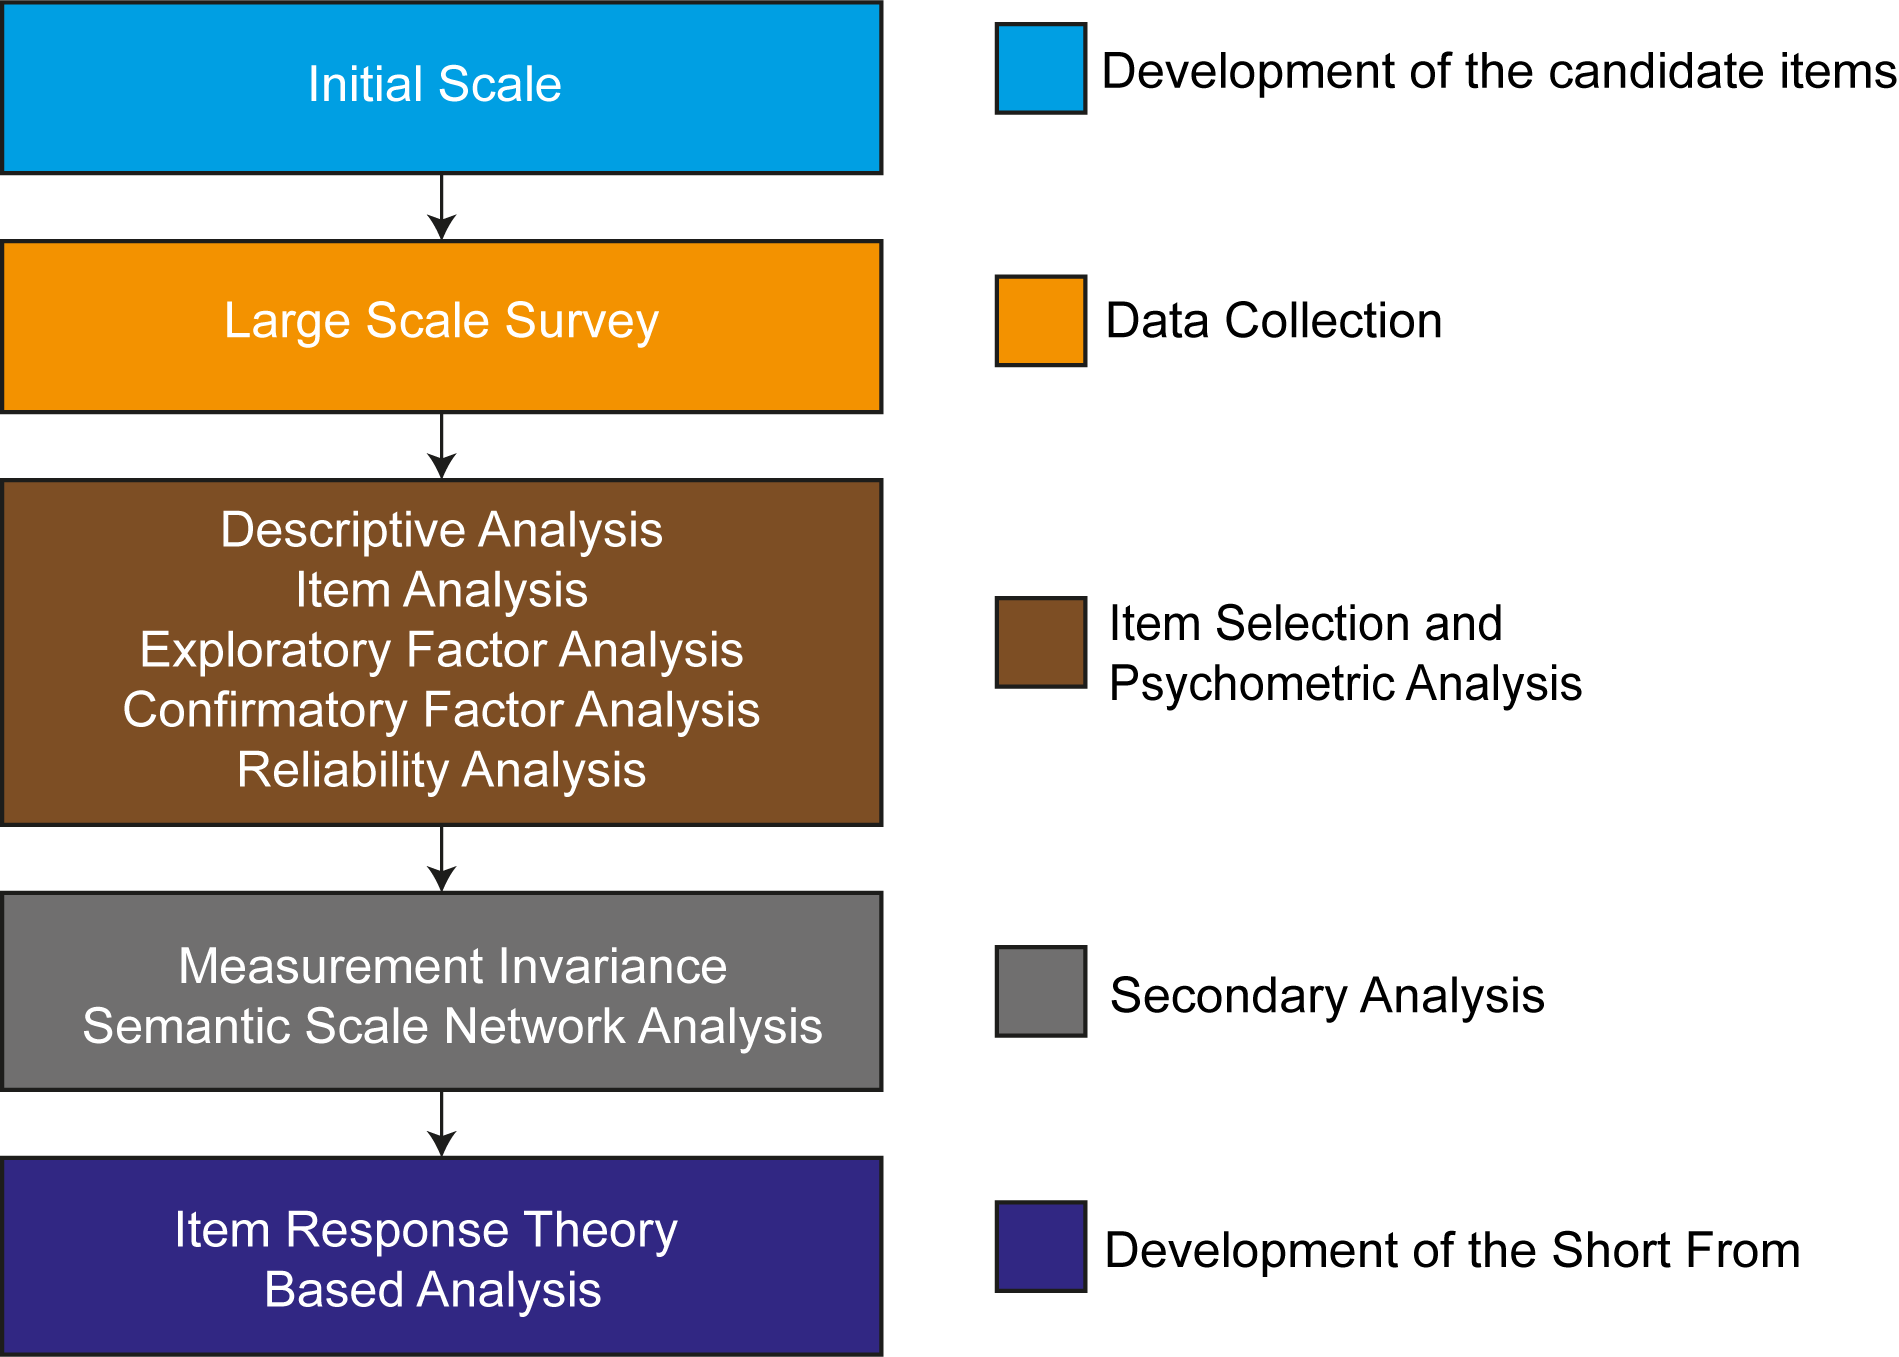
\includegraphics[width=0.5\linewidth,height=0.5\textheight]{Figures/Figure1} 

}

\caption{Flow chart of the LEBA (long and short form) development and evaluation. }\label{fig:FlowchartFig}
\end{figure}

\hypertarget{ethical-approval}{%
\subsection{Ethical approval}\label{ethical-approval}}

The current research project utilizes fully anonymous online survey data and therefore does not fall under the scope of the Human Research Act, making an authorisation from the ethics committee redundant. Nevertheless, the cantonal ethics commission (Ethikkommission Nordwest- und Zentralschweiz, EKNZ) reviewed our proposition (project ID Req-2021-00488) and issued an official clarification of responsibility.

\hypertarget{code-materials-and-data-availability}{%
\subsection{Code, materials and data availability}\label{code-materials-and-data-availability}}

The present article is a fully reproducible open access ``R Markdown'' document. All code and data underlying this article is available on a public \href{https://github.com/leba-instrument}{GitHub repository}. The English version of long and short form of LEBA inventory and online survey implementation templates on common survey platforms (Qualtrics and REDCap) -- is available on another public \href{https://github.com/leba-instrument/leba-instrument-en}{GitHub repository} as well as on the dedicated \href{https://leba-instrument.org/}{website} of the LEBA inventory under an open-access licence (Creative Commons CC-BY-NC-ND).

\newpage

\hypertarget{references}{%
\section{References}\label{references}}

\begingroup
\setlength{\parindent}{-0.5in}
\setlength{\leftskip}{0.5in}

\hypertarget{refs}{}
\begin{CSLReferences}{0}{0}
\leavevmode\vadjust pre{\hypertarget{ref-boyce_light_2022}{}}%
\CSLLeftMargin{1. }%
\CSLRightInline{Boyce, P. \href{https://doi.org/10.1177/14771535211010267}{Light, lighting and human health}. \emph{Lighting Research \& Technology} \textbf{54}, 101--144 (2022).}

\leavevmode\vadjust pre{\hypertarget{ref-blume_effects_2019}{}}%
\CSLLeftMargin{2. }%
\CSLRightInline{Blume, C., Garbazza, C. \& Spitschan, M. \href{https://doi.org/10.1007/s11818-019-00215-x}{Effects of light on human circadian rhythms, sleep and mood}. \emph{Somnologie : Schlafforschung und Schlafmedizin = Somnology : sleep research and sleep medicine} \textbf{23}, 147--156 (2019).}

\leavevmode\vadjust pre{\hypertarget{ref-Klepeis.2001}{}}%
\CSLLeftMargin{3. }%
\CSLRightInline{Klepeis, N. E. \emph{et al.} \href{https://doi.org/10.1038/sj.jea.7500165}{The national human activity pattern survey (NHAPS): A resource for assessing exposure to environmental pollutants}. \emph{Journal of exposure analysis and environmental epidemiology} \textbf{11}, 231--252 (2001).}

\leavevmode\vadjust pre{\hypertarget{ref-navara2007dark}{}}%
\CSLLeftMargin{4. }%
\CSLRightInline{Navara, K. J. \& Nelson, R. J. The dark side of light at night: Physiological, epidemiological, and ecological consequences. \emph{Journal of pineal research} \textbf{43}, 215--224 (2007).}

\leavevmode\vadjust pre{\hypertarget{ref-Lunn.2017}{}}%
\CSLLeftMargin{5. }%
\CSLRightInline{Lunn, R. M. \emph{et al.} \href{https://doi.org/10.1016/j.scitotenv.2017.07.056}{Health consequences of electric lighting practices in the modern world: A report on the national toxicology program's workshop on shift work at night, artificial light at night, and circadian disruption}. \emph{The Science of the total environment} \textbf{607-608}, 1073--1084 (2017).}

\leavevmode\vadjust pre{\hypertarget{ref-Chellappa.2019}{}}%
\CSLLeftMargin{6. }%
\CSLRightInline{Chellappa, S. L., Vujovic, N., Williams, J. S. \& Scheer, F. A. J. L. \href{https://doi.org/10.1016/j.tem.2019.07.008}{Impact of circadian disruption on cardiovascular function and disease}. \emph{Trends in endocrinology and metabolism: TEM} \textbf{30}, 767--779 (2019).}

\leavevmode\vadjust pre{\hypertarget{ref-Brown.2022}{}}%
\CSLLeftMargin{7. }%
\CSLRightInline{Brown, T. M. \emph{et al.} \href{https://doi.org/10.1371/journal.pbio.3001571}{Recommendations for daytime, evening, and nighttime indoor light exposure to best support physiology, sleep, and wakefulness in healthy adults}. \emph{PLoS biology} \textbf{20}, e3001571 (2022).}

\leavevmode\vadjust pre{\hypertarget{ref-hubalek_ambulant_2006}{}}%
\CSLLeftMargin{8. }%
\CSLRightInline{Hubalek, S., Zöschg, D. \& Schierz, C. \href{https://doi.org/10.1177/1477153506070687}{Ambulant recording of light for vision and non-visual biological effects}. \emph{Lighting Research \& Technology} \textbf{38}, 314--321 (2006).}

\leavevmode\vadjust pre{\hypertarget{ref-hartmeyer2022towards}{}}%
\CSLLeftMargin{9. }%
\CSLRightInline{Hartmeyer, S. L., Webler, F. S. \& Andersen, M. Towards a framework for light-dosimetry studies: Methodological considerations. \emph{Lighting Research \& Technology} 14771535221103258 (2022).}

\leavevmode\vadjust pre{\hypertarget{ref-spitschan2022verification}{}}%
\CSLLeftMargin{10. }%
\CSLRightInline{Spitschan, M. \emph{et al.} Verification, analytical validation and clinical validation (V3) of wearable dosimeters and light loggers. \emph{Digital Health} \textbf{8}, 20552076221144858 (2022).}

\leavevmode\vadjust pre{\hypertarget{ref-hurvich_perception_1966}{}}%
\CSLLeftMargin{11. }%
\CSLRightInline{Hurvich, L. M. \& Jameson, D. \emph{The perception of brightness and darkness}. (1966).}

\leavevmode\vadjust pre{\hypertarget{ref-allen_exploiting_2018}{}}%
\CSLLeftMargin{12. }%
\CSLRightInline{Allen, A. E., Hazelhoff, E. M., Martial, F. P., Cajochen, C. \& Lucas, R. J. \href{https://doi.org/10.1093/sleep/zsy100}{Exploiting metamerism to regulate the impact of a visual display on alertness and melatonin suppression independent of visual appearance}. \emph{Sleep} \textbf{41}, zsy100 (2018).}

\leavevmode\vadjust pre{\hypertarget{ref-shapiroAnalysisVarianceTest1965}{}}%
\CSLLeftMargin{13. }%
\CSLRightInline{Shapiro, S. S. \& Wilk, M. B. \href{https://doi.org/10.1093/biomet/52.3-4.591}{An analysis of variance test for normality (complete samples)}. \emph{Biometrika} \textbf{52}, 591--611 (1965).}

\leavevmode\vadjust pre{\hypertarget{ref-mardiaMeasuresMultivariateSkewness1970}{}}%
\CSLLeftMargin{14. }%
\CSLRightInline{Mardia, K. V. \href{https://doi.org/10.1093/biomet/57.3.519}{Measures of multivariate skewness and kurtosis with applications}. \emph{Biometrika} \textbf{57}, 519--530 (1970).}

\leavevmode\vadjust pre{\hypertarget{ref-kaiserIndexFactorialSimplicity1974}{}}%
\CSLLeftMargin{15. }%
\CSLRightInline{Kaiser, H. F. \href{https://doi.org/10.1007/bf02291575}{An index of factorial simplicity}. \emph{Psychometrika} \textbf{39}, 31--36 (1974).}

\leavevmode\vadjust pre{\hypertarget{ref-bartlettNoteMultiplyingFactors1954}{}}%
\CSLLeftMargin{16. }%
\CSLRightInline{Bartlett, M. A {Note} on the {Multiplying Factors} for {Various Chi}-square {Approximations}. \emph{Journal of the Royal Statistical Society. Series B, Methodological} \textbf{16}, 296--298 (1954).}

\leavevmode\vadjust pre{\hypertarget{ref-hutchesonMultivariateSocialScientist1999}{}}%
\CSLLeftMargin{17. }%
\CSLRightInline{Hutcheson, G. D. \emph{The multivariate social scientist : Introductory statistics using generalized linear models}. ({London : SAGE}, 1999).}

\leavevmode\vadjust pre{\hypertarget{ref-velicerDeterminingNumberComponents1976}{}}%
\CSLLeftMargin{18. }%
\CSLRightInline{Velicer, W. \href{https://doi.org/10.1007/BF02293557}{Determining the {Number} of {Components} from the {Matrix} of {Partial Correlations}}. \emph{Psychometrika} \textbf{41}, 321--327 (1976).}

\leavevmode\vadjust pre{\hypertarget{ref-lorenzo-sevaHullMethodSelecting2011}{}}%
\CSLLeftMargin{19. }%
\CSLRightInline{Lorenzo-Seva, U., Timmerman, M. \& Kiers, H. \href{https://doi.org/10.1080/00273171.2011.564527}{The {Hull Method} for {Selecting} the {Number} of {Common Factors}}. \emph{Multivariate Behavioral Research} \textbf{46}, 340--364 (2011).}

\leavevmode\vadjust pre{\hypertarget{ref-desjardinsHandbookEducationalMeasurement2018}{}}%
\CSLLeftMargin{20. }%
\CSLRightInline{Desjardins, C. \& Bulut, O. \emph{Handbook of {Educational Measurement} and {Psychometrics Using R}}. ({Chapman and Hall/CRC}, 2018). doi:\href{https://doi.org/10.1201/b20498}{10.1201/b20498}.}

\leavevmode\vadjust pre{\hypertarget{ref-flesch1948new}{}}%
\CSLLeftMargin{21. }%
\CSLRightInline{Flesch, R. A new readability yardstick. \emph{Journal of applied psychology} \textbf{32}, 221 (1948).}

\leavevmode\vadjust pre{\hypertarget{ref-rosenbusch2020semantic}{}}%
\CSLLeftMargin{22. }%
\CSLRightInline{Rosenbusch, H., Wanders, F. \& Pit, I. L. The semantic scale network: An online tool to detect semantic overlap of psychological scales and prevent scale redundancies. \emph{Psychological methods} \textbf{25}, 380 (2020).}

\leavevmode\vadjust pre{\hypertarget{ref-bruni1996sleep}{}}%
\CSLLeftMargin{23. }%
\CSLRightInline{Bruni, O. \emph{et al.} The sleep disturbance scale for children (SDSC) construct ion and validation of an instrument to evaluate sleep disturbances in childhood and adolescence. \emph{Journal of sleep research} \textbf{5}, 251--261 (1996).}

\leavevmode\vadjust pre{\hypertarget{ref-robins1988composite}{}}%
\CSLLeftMargin{24. }%
\CSLRightInline{Robins, L. N. \emph{et al.} The composite international diagnostic interview: An epidemiologic instrument suitable for use in conjunction with different diagnostic systems and in different cultures. \emph{Archives of general psychiatry} \textbf{45}, 1069--1077 (1988).}

\leavevmode\vadjust pre{\hypertarget{ref-samejima1997handbook}{}}%
\CSLLeftMargin{25. }%
\CSLRightInline{Samejima, F., Liden, W. van der \& Hambleton, R. Handbook of modern item response theory. (1997).}

\leavevmode\vadjust pre{\hypertarget{ref-bakerBasicsItemResponse2017}{}}%
\CSLLeftMargin{26. }%
\CSLRightInline{Baker, F. B. \& Kim, S.-H. \emph{The basics of item response theory using r}. (Springer, 2017).}

\leavevmode\vadjust pre{\hypertarget{ref-dall2010developmental}{}}%
\CSLLeftMargin{27. }%
\CSLRightInline{Dall'Oglio, A. M. \emph{et al.} Developmental evaluation at age 4: Validity of an italian parental questionnaire. \emph{Journal of paediatrics and child health} \textbf{46}, 419--426 (2010).}

\leavevmode\vadjust pre{\hypertarget{ref-field2013discovering}{}}%
\CSLLeftMargin{28. }%
\CSLRightInline{Field, A. \emph{Discovering statistics using IBM SPSS statistics}. (sage, 2015).}

\leavevmode\vadjust pre{\hypertarget{ref-Nunnally1978}{}}%
\CSLLeftMargin{29. }%
\CSLRightInline{Nunnally, J. C. \emph{Psychometric theory}. ({McGraw-Hill}, 1978).}

\leavevmode\vadjust pre{\hypertarget{ref-santhi_applications_2020}{}}%
\CSLLeftMargin{30. }%
\CSLRightInline{Santhi, N. \& Ball, D. M. \href{https://doi.org/10.1016/bs.pbr.2020.05.029}{Applications in sleep: {How} light affects sleep}. \emph{Progress in brain research} \textbf{253}, 17--24 (2020).}

\leavevmode\vadjust pre{\hypertarget{ref-thomas2019advances}{}}%
\CSLLeftMargin{31. }%
\CSLRightInline{Thomas, M. L. Advances in applications of item response theory to clinical assessment. \emph{Psychological assessment} \textbf{31}, 1442 (2019).}

\leavevmode\vadjust pre{\hypertarget{ref-lok2018light}{}}%
\CSLLeftMargin{32. }%
\CSLRightInline{Lok, R., Smolders, K. C., Beersma, D. G. \& de Kort, Y. A. Light, alertness, and alerting effects of white light: A literature overview. \emph{Journal of biological rhythms} \textbf{33}, 589--601 (2018).}

\leavevmode\vadjust pre{\hypertarget{ref-siraji2021effects}{}}%
\CSLLeftMargin{33. }%
\CSLRightInline{Siraji, M. A., Kalavally, V., Schaefer, A. \& Haque, S. Effects of daytime electric light exposure on human alertness and higher cognitive functions: A systematic review. \emph{Frontiers in psychology} \textbf{12}, 765750--765750 (2021).}

\leavevmode\vadjust pre{\hypertarget{ref-Siraji.2023}{}}%
\CSLLeftMargin{34. }%
\CSLRightInline{Siraji, M. A., Spitschan, M., Kalavally, V. \& Haque, S. \href{https://doi.org/10.1038/s41598-023-39636-y}{Light exposure behaviors predict mood, memory and sleep quality}. \emph{Scientific Reports} \textbf{13}, 12425 (2023).}

\leavevmode\vadjust pre{\hypertarget{ref-harris2009research}{}}%
\CSLLeftMargin{35. }%
\CSLRightInline{Harris, P. A. \emph{et al.} Research electronic data capture (REDCap)---a metadata-driven methodology and workflow process for providing translational research informatics support. \emph{Journal of biomedical informatics} \textbf{42}, 377--381 (2009).}

\leavevmode\vadjust pre{\hypertarget{ref-harris2019redcap}{}}%
\CSLLeftMargin{36. }%
\CSLRightInline{Harris, P. A. \emph{et al.} The REDCap consortium: Building an international community of software platform partners. \emph{Journal of biomedical informatics} \textbf{95}, 103208 (2019).}

\leavevmode\vadjust pre{\hypertarget{ref-Weinzaepflen.2021}{}}%
\CSLLeftMargin{37. }%
\CSLRightInline{Weinzaepflen, C. \& Spitschan, M. Enlighten your clock: How your body tells time. (2021) doi:\href{https://doi.org/10.17605/OSF.IO/ZQXVH}{10.17605/OSF.IO/ZQXVH}.}

\leavevmode\vadjust pre{\hypertarget{ref-f.lux}{}}%
\CSLLeftMargin{38. }%
\CSLRightInline{F.lux Software LLC. \href{https://justgetflux.com/}{F.lux}. (2021).}

\leavevmode\vadjust pre{\hypertarget{ref-comreyFirstCourseFactor1992}{}}%
\CSLLeftMargin{39. }%
\CSLRightInline{Comrey, A. L. \& Lee, H. B. \emph{A first course in factor analysis}. (Psychology press, 2013).}

\leavevmode\vadjust pre{\hypertarget{ref-schonbrodtWhatSampleSize2013}{}}%
\CSLLeftMargin{40. }%
\CSLRightInline{Schönbrodt, F. D. \& Perugini, M. \href{https://doi.org/10.1016/j.jrp.2013.05.009}{At what sample size do correlations stabilize?} \emph{Journal of research in personality} \textbf{47}, 609--612 (2013).}

\leavevmode\vadjust pre{\hypertarget{ref-bentlerPracticalIssuesStructural1987}{}}%
\CSLLeftMargin{41. }%
\CSLRightInline{Bentler, P. M. \& Chou, C.-P. \href{https://doi.org/10.1177/0049124187016001004}{Practical {Issues} in {Structural Modeling}}. \emph{Sociological methods \& research} \textbf{16}, 78--117 (1987).}

\leavevmode\vadjust pre{\hypertarget{ref-jacksonRevisitingSampleSize2003}{}}%
\CSLLeftMargin{42. }%
\CSLRightInline{Jackson, D. L. \href{https://doi.org/10.1207/S15328007SEM1001_6}{Revisiting {Sample Size} and {Number} of {Parameter Estimates}: {Some Support} for the {N}:q {Hypothesis}}. \emph{Structural equation modeling} \textbf{10}, 128--141 (2003).}

\leavevmode\vadjust pre{\hypertarget{ref-klinePrinciplesPracticeStructural2015}{}}%
\CSLLeftMargin{43. }%
\CSLRightInline{Kline, R. B. \emph{Principles and practice of structural equation modeling}. ({The Guilford Press}, 2016).}

\leavevmode\vadjust pre{\hypertarget{ref-worthingtonScaleDevelopmentResearch2006}{}}%
\CSLLeftMargin{44. }%
\CSLRightInline{Worthington, R. L. \& Whittaker, T. A. \href{https://doi.org/10.1177/0011000006288127}{Scale {Development Research}: {A Content Analysis} and {Recommendations} for {Best Practices}}. \emph{The Counseling psychologist} \textbf{34}, 806--838 (2006).}

\leavevmode\vadjust pre{\hypertarget{ref-watkinsStepbyStepGuideExploratory2020}{}}%
\CSLLeftMargin{45. }%
\CSLRightInline{Watkins, M. \emph{A {Step}-by-{Step Guide} to {Exploratory Factor Analysis} with {R} and {RStudio}}. (2020). doi:\href{https://doi.org/10.4324/9781003120001}{10.4324/9781003120001}.}

\leavevmode\vadjust pre{\hypertarget{ref-cattellScreeTestNumber1966}{}}%
\CSLLeftMargin{46. }%
\CSLRightInline{Cattell, R. B. \href{https://doi.org/10.1207/s15327906mbr0102_10}{The {Scree Test For The Number Of Factors}}. \emph{Multivariate Behavioral Research} \textbf{1}, 245--276 (1966).}

\leavevmode\vadjust pre{\hypertarget{ref-bandalosFactorAnalysisExploratory2018}{}}%
\CSLLeftMargin{47. }%
\CSLRightInline{Bandalos, D. L. \& Finney, S. J. Factor analysis: {Exploratory} and confirmatory. in \emph{The reviewer's guide to quantitative methods in the social sciences} 98--122 ({Routledge}, 2018).}

\leavevmode\vadjust pre{\hypertarget{ref-gadermann2012estimating}{}}%
\CSLLeftMargin{48. }%
\CSLRightInline{Gadermann, A. M., Guhn, M. \& Zumbo, B. D. Estimating ordinal reliability for likert-type and ordinal item response data: A conceptual, empirical, and practical guide. \emph{Practical Assessment, Research, and Evaluation} \textbf{17}, 3 (2012).}

\leavevmode\vadjust pre{\hypertarget{ref-zumbo2007ordinal}{}}%
\CSLLeftMargin{49. }%
\CSLRightInline{Zumbo, B. D., Gadermann, A. M. \& Zeisser, C. Ordinal versions of coefficients alpha and theta for likert rating scales. \emph{Journal of modern applied statistical methods} \textbf{6}, 4 (2007).}

\leavevmode\vadjust pre{\hypertarget{ref-dunn2014alpha}{}}%
\CSLLeftMargin{50. }%
\CSLRightInline{Dunn, T. J., Baguley, T. \& Brunsden, V. From alpha to omega: A practical solution to the pervasive problem of internal consistency estimation. \emph{British journal of psychology} \textbf{105}, 399--412 (2014).}

\leavevmode\vadjust pre{\hypertarget{ref-sijtsma2009use}{}}%
\CSLLeftMargin{51. }%
\CSLRightInline{Sijtsma, K. On the use, the misuse, and the very limited usefulness of cronbach's alpha. \emph{Psychometrika} \textbf{74}, 107 (2009).}

\leavevmode\vadjust pre{\hypertarget{ref-huCutoffCriteriaFit1999}{}}%
\CSLLeftMargin{52. }%
\CSLRightInline{Hu, L. \& Bentle, P. M. \href{https://doi.org/10.1080/10705519909540118}{Cutoff criteria for fit indexes in covariance structure analysis: {Conventional} criteria versus new alternatives}. \emph{Structural Equation Modeling: A Multidisciplinary Journal} \textbf{6}, 1--55 (1999).}

\leavevmode\vadjust pre{\hypertarget{ref-schumacker2004beginner}{}}%
\CSLLeftMargin{53. }%
\CSLRightInline{Schumacker, R. E. \& Lomax, R. G. \emph{A beginner's guide to structural equation modeling}. (psychology press, 2004).}

\leavevmode\vadjust pre{\hypertarget{ref-brownConfirmatoryFactorAnalysis2015}{}}%
\CSLLeftMargin{54. }%
\CSLRightInline{Brown, T. A. \emph{Confirmatory factor analysis for applied research}. ({The Guilford Press}, 2015).}

\leavevmode\vadjust pre{\hypertarget{ref-RN1272}{}}%
\CSLLeftMargin{55. }%
\CSLRightInline{Yu, C. Evaluating cutoff criteria of model fit indices for latent variable models with binary and continuous outcomes. ({ProQuest Dissertations Publishing}, 2002).}

\leavevmode\vadjust pre{\hypertarget{ref-putnick2016measurement}{}}%
\CSLLeftMargin{56. }%
\CSLRightInline{Putnick, D. L. \& Bornstein, M. H. Measurement invariance conventions and reporting: The state of the art and future directions for psychological research. \emph{Developmental review} \textbf{41}, 71--90 (2016).}

\leavevmode\vadjust pre{\hypertarget{ref-dimitrov2010testing}{}}%
\CSLLeftMargin{57. }%
\CSLRightInline{Dimitrov, D. M. Testing for factorial invariance in the context of construct validation. \emph{Measurement and Evaluation in Counseling and Development} \textbf{43}, 121--149 (2010).}

\leavevmode\vadjust pre{\hypertarget{ref-widaman1997exploring}{}}%
\CSLLeftMargin{58. }%
\CSLRightInline{Widaman, K. F. \& Reise, S. P. Exploring the measurement invariance of psychological instruments: Applications in the substance use domain. (1997).}

\leavevmode\vadjust pre{\hypertarget{ref-drasgow1985appropriateness}{}}%
\CSLLeftMargin{59. }%
\CSLRightInline{Drasgow, F., Levine, M. V. \& Williams, E. A. Appropriateness measurement with polychotomous item response models and standardized indices. \emph{British Journal of Mathematical and Statistical Psychology} \textbf{38}, 67--86 (1985).}

\leavevmode\vadjust pre{\hypertarget{ref-verriotto2017new}{}}%
\CSLLeftMargin{60. }%
\CSLRightInline{Verriotto, J. D. \emph{et al.} New methods for quantification of visual photosensitivity threshold and symptoms. \emph{Translational vision science \& technology} \textbf{6}, 18--18 (2017).}

\leavevmode\vadjust pre{\hypertarget{ref-eklund1996development}{}}%
\CSLLeftMargin{61. }%
\CSLRightInline{Eklund, N. \& Boyce, P. The development of a reliable, valid, and simple office lighting survey. \emph{Journal of the Illuminating Engineering Society} \textbf{25}, 25--40 (1996).}

\leavevmode\vadjust pre{\hypertarget{ref-bajaj2011validation}{}}%
\CSLLeftMargin{62. }%
\CSLRightInline{Bajaj, A., Rosner, B., Lockley, S. W. \& Schernhammer, E. S. Validation of a light questionnaire with real-life photopic illuminance measurements: The harvard light exposure assessment questionnaire. \emph{Cancer Epidemiology and Prevention Biomarkers} \textbf{20}, 1341--1349 (2011).}

\leavevmode\vadjust pre{\hypertarget{ref-dianat2013objective}{}}%
\CSLLeftMargin{63. }%
\CSLRightInline{Dianat, I., Sedghi, A., Bagherzade, J., Jafarabadi, M. A. \& Stedmon, A. W. Objective and subjective assessments of lighting in a hospital setting: Implications for health, safety and performance. \emph{Ergonomics} \textbf{56}, 1535--1545 (2013).}

\leavevmode\vadjust pre{\hypertarget{ref-horne1976self}{}}%
\CSLLeftMargin{64. }%
\CSLRightInline{Horne, J. A. \& Östberg, O. A self-assessment questionnaire to determine morningness-eveningness in human circadian rhythms. \emph{International journal of chronobiology} (1976).}

\leavevmode\vadjust pre{\hypertarget{ref-roenneberg2003life}{}}%
\CSLLeftMargin{65. }%
\CSLRightInline{Roenneberg, T., Wirz-Justice, A. \& Merrow, M. Life between clocks: Daily temporal patterns of human chronotypes. \emph{Journal of biological rhythms} \textbf{18}, 80--90 (2003).}

\leavevmode\vadjust pre{\hypertarget{ref-grandner2014development}{}}%
\CSLLeftMargin{66. }%
\CSLRightInline{Grandner, M. A., Jackson, N., Gooneratne, N. S. \& Patel, N. P. The development of a questionnaire to assess sleep-related practices, beliefs, and attitudes. \emph{Behavioral sleep medicine} \textbf{12}, 123--142 (2014).}

\leavevmode\vadjust pre{\hypertarget{ref-buysse1989pittsburgh}{}}%
\CSLLeftMargin{67. }%
\CSLRightInline{Buysse, D. J., Reynolds III, C. F., Monk, T. H., Berman, S. R. \& Kupfer, D. J. The pittsburgh sleep quality index: A new instrument for psychiatric practice and research. \emph{Psychiatry research} \textbf{28}, 193--213 (1989).}

\leavevmode\vadjust pre{\hypertarget{ref-Xie.2021}{}}%
\CSLLeftMargin{68. }%
\CSLRightInline{Xie, Y., Wu, X., Tao, S., Wan, Y. \& Tao, F. Development and validation of the self-rating of biological rhythm disorder for chinese adolescents. \emph{Chronobiology International} 1--7 (2022) doi:\href{https://doi.org/10.1080/07420528.2021.1989450}{10.1080/07420528.2021.1989450}.}

\leavevmode\vadjust pre{\hypertarget{ref-bossini2006sensibilita}{}}%
\CSLLeftMargin{69. }%
\CSLRightInline{Bossini, L. \emph{et al.} Sensibilit{à} alla luce e psicopatologia: Validazione del questionario per la valutazione della fotosensibilit{à} (QVF). \emph{Med Psicosomatica} \textbf{51}, 167--176 (2006).}

\end{CSLReferences}

\endgroup


\end{document}
